\documentclass[UTF8,12pt,a4paper]{ctexart}

\usepackage{amsmath,amssymb,bm}
\usepackage{booktabs,longtable,array}
\usepackage{geometry}
\usepackage{graphicx}
\usepackage{float}
\usepackage{caption}
\usepackage[hidelinks]{hyperref}
\usepackage{xcolor}
\usepackage{url}
\geometry{left=2.5cm,right=2.5cm,top=2.5cm,bottom=2.5cm}
\graphicspath{{figs/}}
\captionsetup{font=small,labelsep=quad}
\setlength{\parindent}{2em}
\setlength{\parskip}{0pt}
\linespread{1.22}
\newcommand{\keywords}[1]{\par\noindent\textbf{关键词：}#1}
\newcommand{\dd}{\,\mathrm d}

\title{\textbf{含储能微网的确定性调度、\\因果预测与滚动再调度}}
\author{}
\date{}

\begin{document}
\pagestyle{plain}
\pagenumbering{arabic}
\setcounter{page}{1}
\maketitle

\begin{abstract}
针对光伏、负荷和分时电价共同作用下的微网购电与储能调度问题，本文分别建立单日确定性混合整数线性规划模型和含预测误差的全年因果滚动随机优化模型。建模统一采用10分钟离散时标，将功率换算为区间电量，并显式刻画储能充放电效率、容量与功率边界、充放电互斥、弃光和紧急购电。

对于问题一，以单日购电费用为主目标，在保持最优费用的条件下以储能吞吐量为次目标消除退化解。模型得到计划购电费用 $35126.95$ 元、总购电量 $59482.70$ kWh；与不使用储能且禁止售电的 $48052.05$ 元基线相比，费用降低 $12925.10$ 元，降幅约 $26.90\%$。储电量始终位于闭区间 $[1200,10800]$ kWh 并触及上下界，最大能量平衡残差为 $2.27\times10^{-13}$ kWh，未出现同时充放电。

对于问题二，在每天0:00仅使用此前已发生数据，组合昨日同刻、近7日同刻均值、上周同刻和梯度提升回归，得到未来48小时的因果预测；再从历史样本外残差中抽取整日路径，构建两阶段随机混合整数规划。当天只执行滚动视窗前144段，计划冻结后用实际负荷与光伏回放结算，并把实际日末储电量传递到次日。该机制避免把预测储电量误差逐日累积。2025年2月1日至12月31日共334天、48096个时段的回放总费用为 $14954855.21$ 元，其中计划购电费 $13670139.41$ 元、紧急购电费 $1284715.79$ 元，紧急购电量 $301509.75$ kWh。负荷和光伏日预测平均NMAE分别为 $5.00\%$ 和 $7.04\%$。全年实际能量平衡残差小于 $7\times10^{-13}$ kWh，状态递推残差小于 $6\times10^{-12}$ kWh，跨日状态缺口为0。

受单日求解时限约束，全年实际采用分级回退：30情景主模型62天、10情景模型271天、Q80确定性模型1天。因此本文结果应解释为带显式回退机制的混合执行策略。数值复算、物理约束、因果训练截止日和结果模板均通过独立检查。

对于问题三，比较“预测24小时、执行6小时”和“预测48小时、执行6小时”两种滚动策略。两者每6小时同步更新、使用完全相同的信息集和10条负荷--光伏残差情景，并将增购与退购费用直接纳入目标。334天配对回放中，H24与H48总费用分别为 $15464289.45$ 元和 $15358936.78$ 元，H48节省 $105352.66$ 元，约 $0.681\%$；7日移动块bootstrap得到日均费用差95\%置信区间为 $[258.87,371.89]$ 元/日。因此在本文10情景设定下推荐H48。

对于问题四，引入附件4的波动电价。计划阶段以目标交易日上周同星期同时间的价格作为因果预测，负荷和光伏仍采用10条历史残差情景；结算阶段使用附件4真实价格。问题4-2每日0:00决策一次，H24与H48总费用分别为 $16548003.63$ 元和 $16338121.68$ 元；问题4-3每6小时再调度，两者总费用分别为 $16245477.76$ 元和 $16080198.49$ 元。H48分别节省 $1.268\%$ 和 $1.017\%$，表明较长视窗能改善跨日电量配置，但其求解耗时显著增加。

\keywords{微网调度；储能系统；两阶段随机规划；因果预测；模型预测控制；滚动再调度}
\end{abstract}

\newpage

\section{问题重述与研究思路}

\subsection{问题背景与任务}

微网需要协调外部电网购电、光伏发电和储能系统，以满足负荷需求并降低购电成本。外部电价按10分钟时段变化，储能既能在低价时段吸收能量，也能在高价时段放电；与此同时，光伏的日内集中出力与负荷峰值并不总是同步。若忽略储能状态的跨时段耦合，局部最低价或局部净负荷规则通常不能形成全局可行计划。

问题一给定一天的电价、负荷和光伏预测，要求制定计划购电与储能充放电方案，并满足首末储电量相同。问题二进一步给出全年负荷与光伏实际数据，要求在每天0:00制定计划，预测误差造成的供能缺口需按当时电价5倍紧急购电。问题三允许每6小时调整购电计划，调整后增购按当时电价1.5倍支付，退购按0.5倍返还，要求确定合理的预测长度与滚动策略。问题四把固定电价替换为附件4的全年波动电价，要求重新制定问题二和问题三的购电方案。四问依次由确定输入的单日调度，过渡到负荷与光伏不确定下的全年决策，再引入日内再决策与价格不确定性。

\subsection{总体研究思路}

微网随机优化通常需要联合考虑可再生能源不确定性与储能的时间耦合\cite{liang2014stochastic}。本文按以下逻辑建立递进模型：

\begin{enumerate}
  \item 统一时间、功率和电量口径，把144个10分钟时段记为 $t=0,\ldots,143$；
  \item 在问题一中建立确定性MILP，求得单日费用最优计划，并用次目标消除无意义的储能循环；
  \item 在问题二中构造只使用历史信息的组合预测和残差情景，建立48小时两阶段随机MILP；
  \item 每日只执行视窗前24小时，随后用实际值进行顺序回放，将实际状态传给次日；
  \item 在问题三中每6小时滚动再优化，分别设置24小时和48小时预测窗口，并在同一场景路径下作全年配对比较；
  \item 在问题四中以周滞后价格构造因果电价预测，分别复现每日决策与6小时再调度，并用真实波动电价结算；
  \item 对费用、能量平衡、状态递推、互斥逻辑、因果性和配对公平性进行交叉验证。
\end{enumerate}

\section{模型假设与符号说明}

\subsection{基本假设}

\begin{enumerate}
  \item 每个10分钟区间内电价、负荷功率和光伏功率视为常数，区间长度为 $\Delta t=1/6$ h。
  \item 储能充电效率与放电效率均取 $\eta_c=\eta_d=0.9$；充放电量定义在交流母线侧。
  \item 不允许向外部电网售电。光伏和计划购电超过当期需要的部分记为未利用剩余电量，不产生收入。
  \item 外网计划购电没有题面之外的额外功率上限；储能最大充放电功率为5000 kW。
  \item 问题一采用 $E_0=E_{144}=6000$ kWh。问题二从2025年2月1日开始评价，1月只作为预测历史窗口且储能不参与调度，并将全年实际状态链校准为 $E_{d_0,0}^{\mathrm{real}}=6000$ kWh，其中 $d_0$ 表示2025年2月1日。
  \item 问题二制定第 $d$ 日计划时只能使用严格早于 $d$ 的负荷与光伏数据；第 $d$ 日实际数据只能在计划冻结后用于回放。
  \item 问题三在0:00、6:00、12:00、18:00重新发布计划，每次只执行前6小时；H24与H48除预测窗口长度外采用相同参数和样本路径。
  \item 问题四计划时不能读取目标时段真实电价；实现中以目标日7天前同一时段的实际价格作为预测，真实价格仅在计划锁定后用于费用结算。
\end{enumerate}

\subsection{主要符号}

全文采用的主要符号及单位见表~\ref{tab:symbols}。

\begin{table}[H]
\centering
\caption{主要符号及其含义}
\label{tab:symbols}
\begin{tabular}{>{\centering\arraybackslash}p{2.2cm}p{8.8cm}p{2.2cm}}
\toprule
符号 & 含义 & 单位\\
\midrule
$p_t$ & 第 $t$ 个10分钟时段的电价 & 元/kWh\\
$\widehat p_{d,t},p^{\mathrm{real}}_{d,t}$ & 预测电价、结算用真实电价 & 元/kWh\\
$L_{d,t}$ & 第 $d$ 日第 $t$ 时段负荷功率 & kW\\
$P_{d,t}$ & 第 $d$ 日第 $t$ 时段光伏功率 & kW\\
$g_{d,t}$ & 计划购电量 & kWh\\
$c_{d,t},d_{d,t}$ & 计划充电量、计划放电量（母线侧） & kWh\\
$E_{d,t}$ & 时段开始时储电量 & kWh\\
$h_{d,t}$ & 紧急购电量 & kWh\\
$w_{d,t}$ & 未利用剩余电量 & kWh\\
$z_{d,t}$ & 充放电互斥变量 & --\\
$s$ & 预测误差情景编号 & --\\
$\pi_s$ & 情景概率 & --\\
$k$ & 问题三的日内计划发布序号，$k=0,1,2,3$ & --\\
$u_{d,t}^{(k)},v_{d,t}^{(k)}$ & 第 $k$ 次更新相对旧承诺的增购量、退购量 & kWh\\
$T_H$ & 问题三预测窗口长度，取144或288个时段 & --\\
\bottomrule
\end{tabular}
\end{table}

为简化记号，问题一省略日期下标 $d$。所有进入能量平衡的负荷和光伏功率均先乘 $\Delta t$，避免把kW与kWh直接相加。

\section{问题一：单日确定性储能调度}

\subsection{数据特征与基线}

附件1包含144条记录。电价位于 $0.3713$--$1.3952$ 元/kWh，负荷功率位于 $3309.3934$--$5958.9696$ kW，光伏预测功率位于 $0$--$7612.3160$ kW。全天负荷电量为 $111024.8081$ kWh，光伏预测电量为 $55482.8357$ kWh。图\ref{fig:q1-load-pv}表明，光伏主要集中在白天，而负荷在早晚仍维持较高水平；中午部分时段光伏高于负荷，因此模型必须允许弃光或储能吸收。

\begin{figure}[H]
\centering
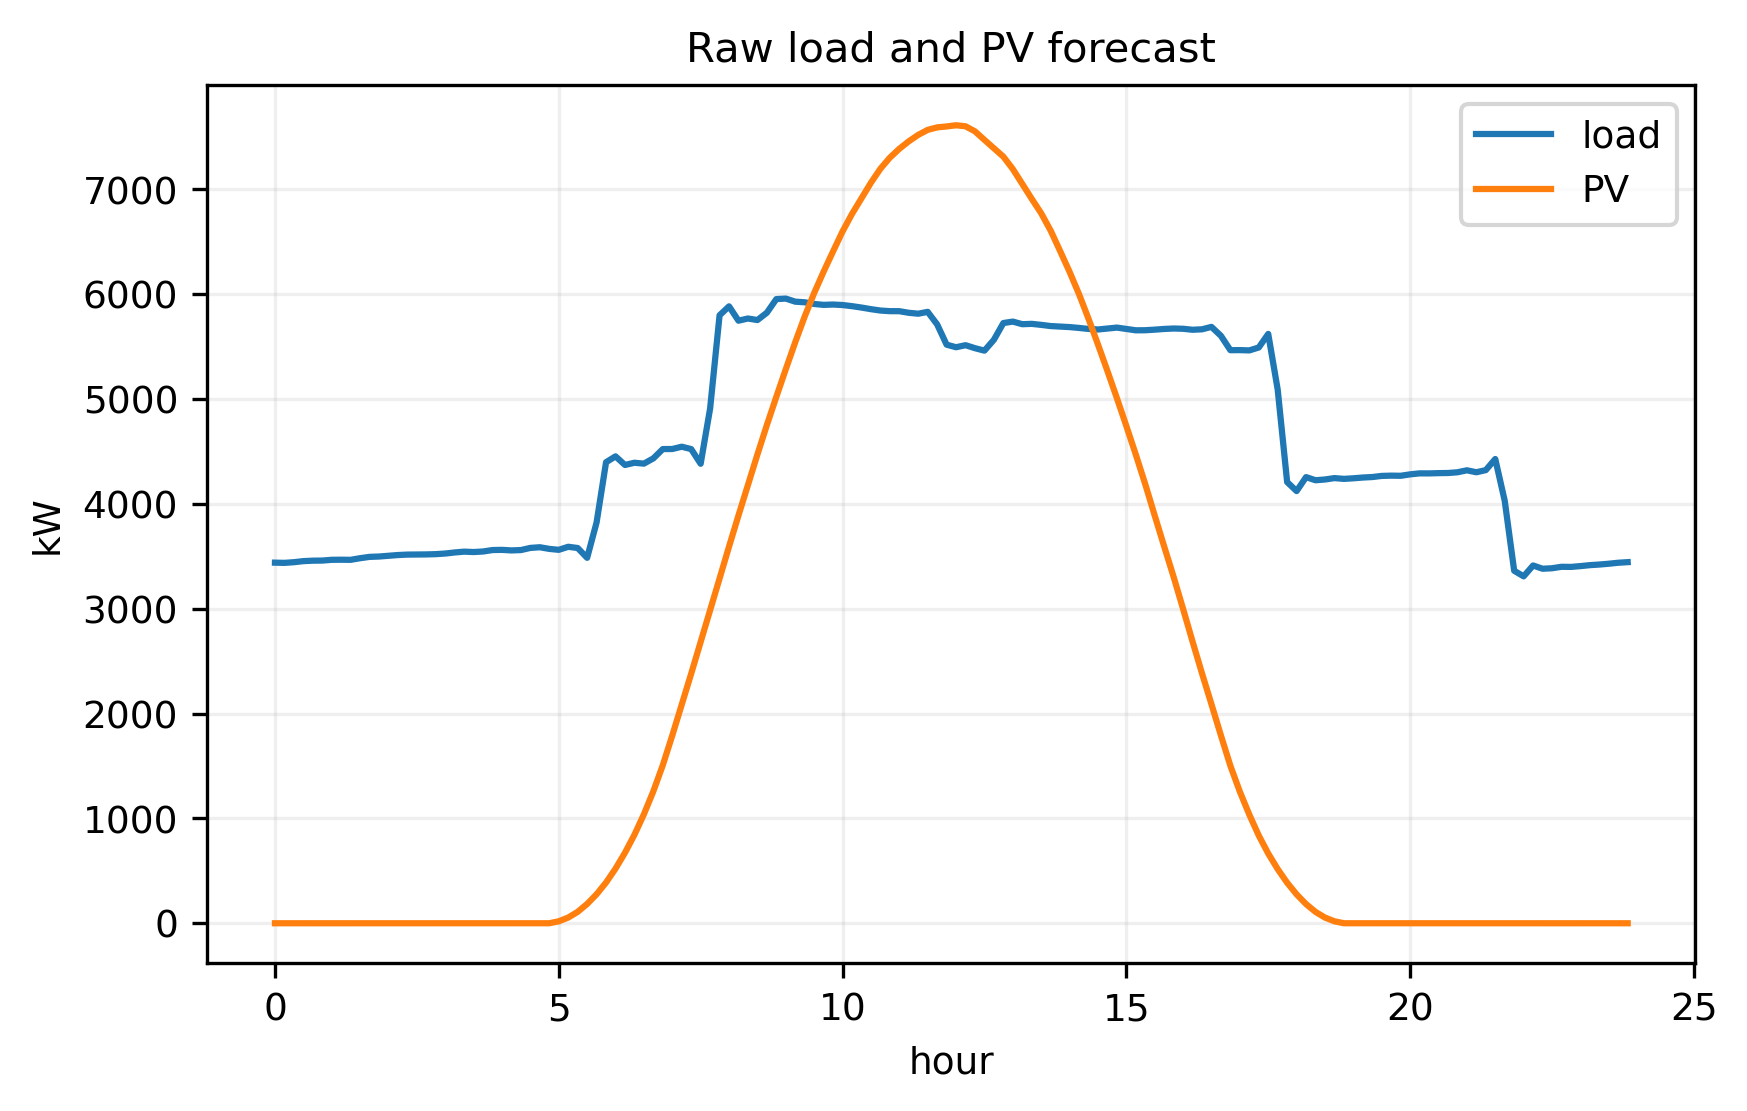
\includegraphics[width=0.88\textwidth]{raw_q1_load_pv.png}
\caption{问题一的负荷与光伏功率曲线}
\label{fig:q1-load-pv}
\end{figure}

若不使用储能且不允许售电，每个时段只购买正净负荷，得到购电费用基线
\begin{equation}
C_{\mathrm{base}}
=\sum_{t=0}^{143}p_t\left[(L_t-P_t)\Delta t\right]_+
=48052.0466\ \text{元}.
\label{eq:q1-baseline}
\end{equation}

\subsection{决策变量与目标函数}

令 $g_t,c_t,d_t,w_t\ge0$ 分别为计划购电量、充电量、放电量和未利用剩余电量，$E_t$ 为储电量，$z_t\in\{0,1\}$ 为充放电模式。第一阶段以购电费用最小为目标：
\begin{equation}
\min C_1=\sum_{t=0}^{143}p_tg_t.
\label{eq:q1-objective}
\end{equation}

只优化式\eqref{eq:q1-objective}时可能存在费用相同但充放电动作不同的退化解。为提高方案可解释性，先取得最优值 $C_1^\star$，再增加 $C_1\le C_1^\star+10^{-6}$，并最小化
\begin{equation}
\min C_2=\sum_{t=0}^{143}(c_t+d_t).
\label{eq:q1-secondary}
\end{equation}
这是一种词典序优化：次目标只在主费用的数值容差内选择储能吞吐量更小的方案，不改变主结论。

\subsection{约束条件}

每个时段满足母线侧能量平衡
\begin{equation}
g_t+P_t\Delta t+d_t=L_t\Delta t+c_t+w_t.
\label{eq:q1-balance}
\end{equation}
储能状态递推为
\begin{equation}
E_{t+1}=E_t+\eta_c c_t-\frac{d_t}{\eta_d}.
\label{eq:q1-state}
\end{equation}
容量和功率约束为
\begin{align}
1200&\le E_t\le10800, \label{eq:q1-energy-bound}\\
0\le c_t&\le \frac{5000}{6}z_t,\qquad
0\le d_t\le \frac{5000}{6}(1-z_t). \label{eq:q1-mode}
\end{align}
式\eqref{eq:q1-mode}利用二元变量排除同时充放电。为保证一天结束后不透支未来，设置
\begin{equation}
E_0=E_{144}=6000.
\label{eq:q1-terminal}
\end{equation}

\subsection{求解方法}

模型含连续变量和二元变量，属于MILP。本文使用Python构造稀疏约束矩阵并调用SciPy的HiGHS接口。HiGHS中的线性规划核心算法具有现代对偶修正单纯形并行实现背景\cite{huangfu2017parallelizing}；本文不据此替代MILP的数值验证，而是另外复算目标函数及全部物理残差。

\subsection{求解结果与分析}

图\ref{fig:q1-dispatch}给出购电、充电和放电的联合时序。储能在低价或光伏富余时段吸收能量，在高价且净负荷为正时放电。图\ref{fig:q1-storage}显示状态轨迹在闭区间内运行并满足首末一致；触及边界意味着容量约束确实影响了最优调度。

\begin{figure}[H]
\centering
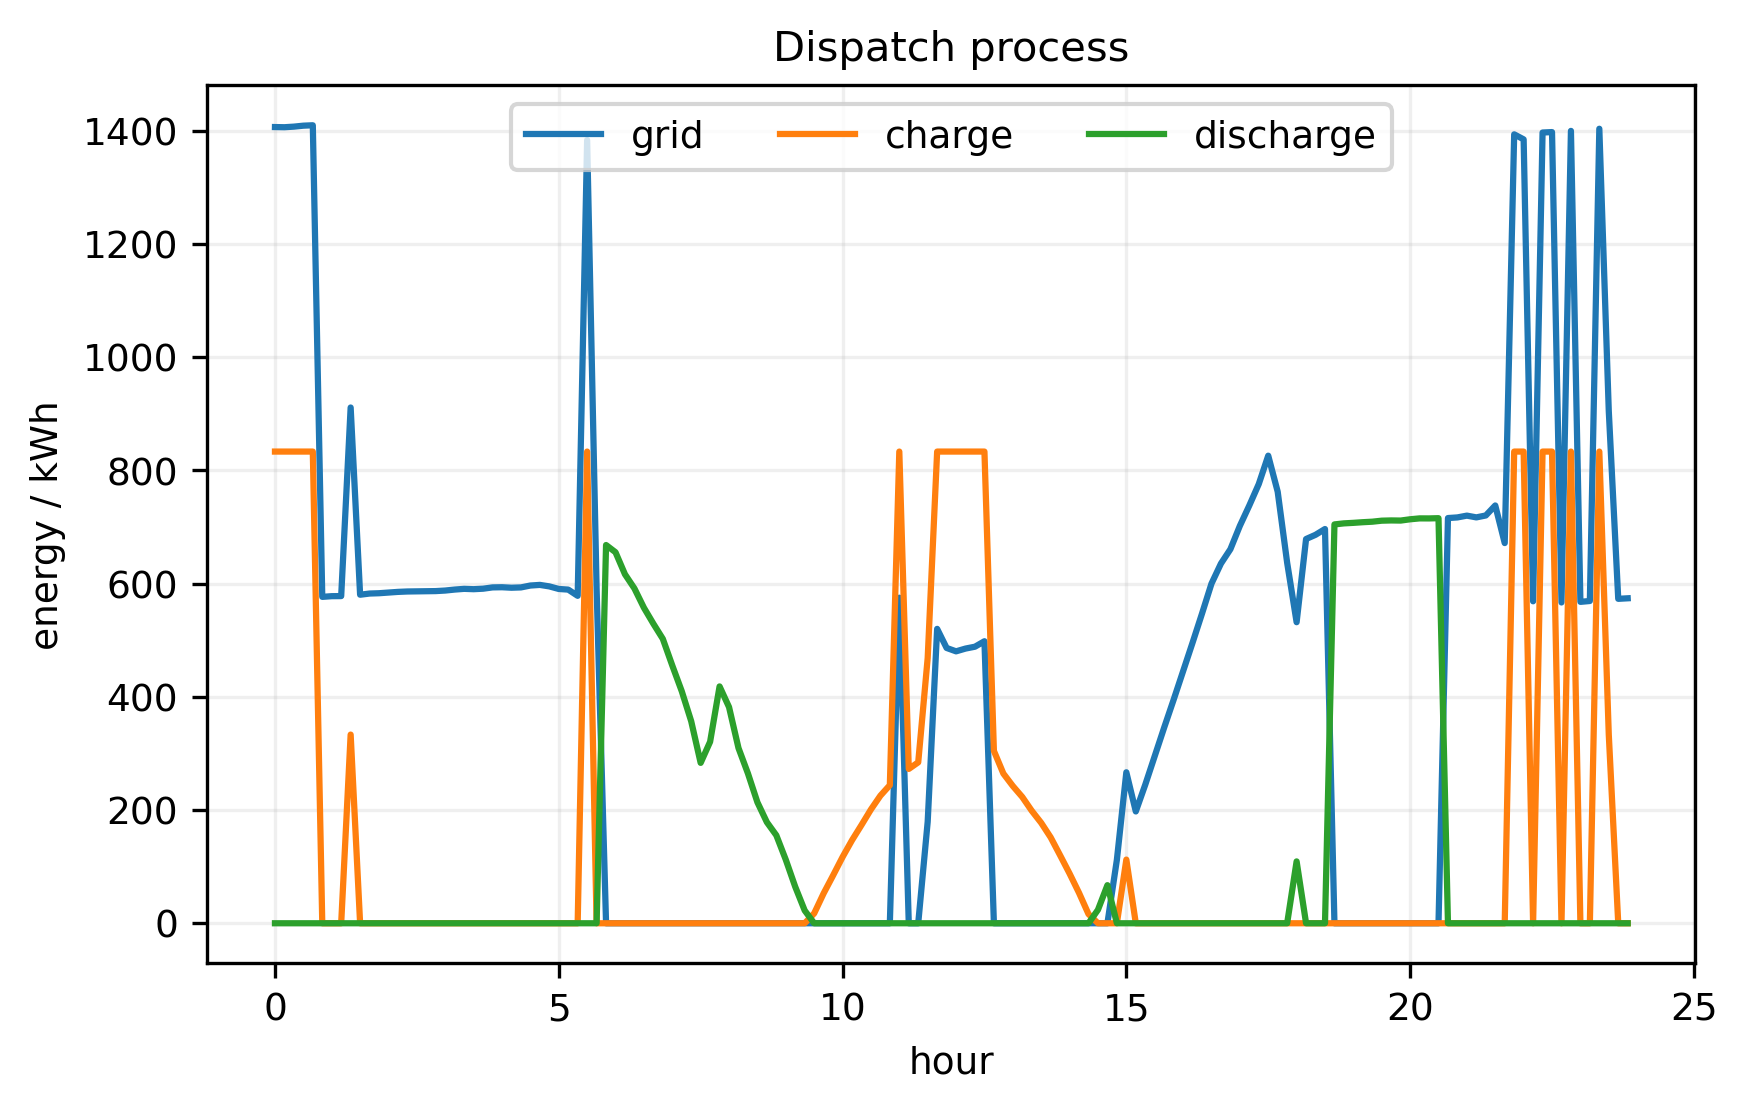
\includegraphics[width=0.90\textwidth]{process_q1_dispatch.png}
\caption{问题一的购电与储能充放电调度}
\label{fig:q1-dispatch}
\end{figure}

\begin{figure}[H]
\centering
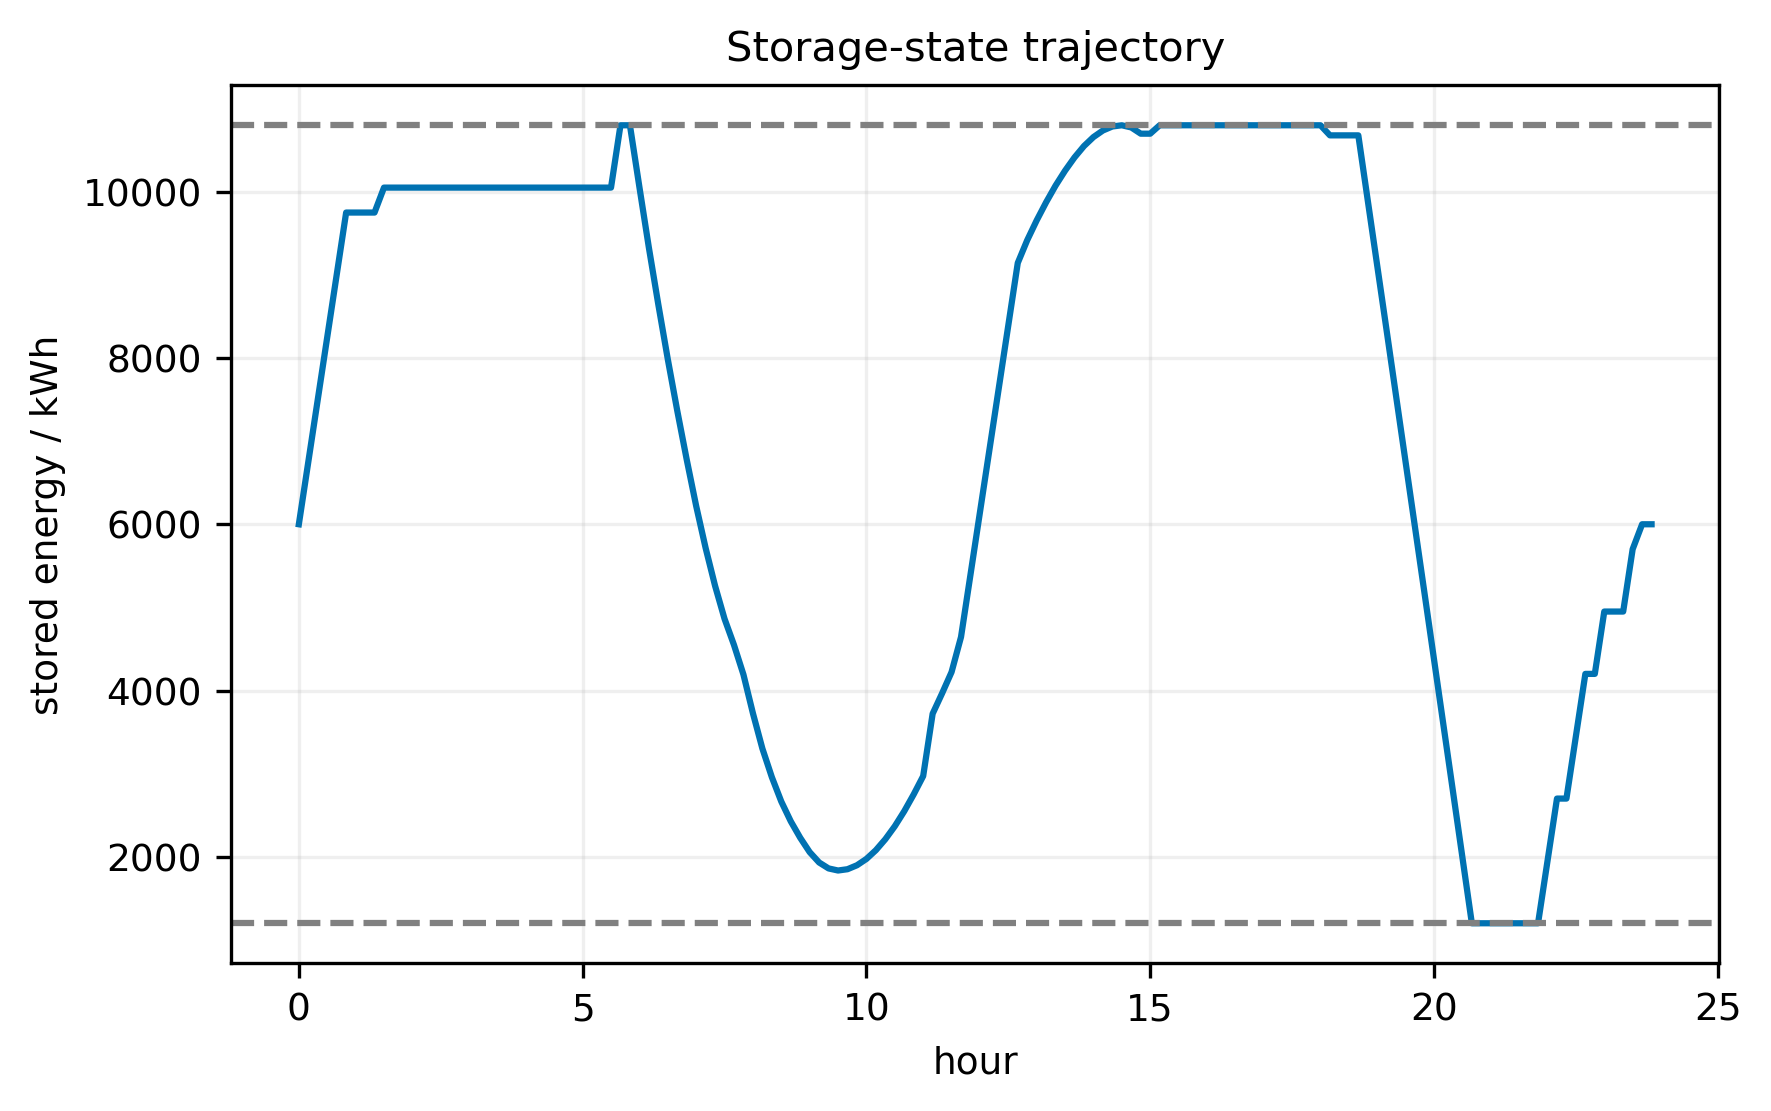
\includegraphics[width=0.90\textwidth]{process_q1_storage.png}
\caption{问题一的储电量状态轨迹}
\label{fig:q1-storage}
\end{figure}

关键结果列于表\ref{tab:q1-results}。主目标与二阶段固定后的费用差仅为 $1.00\times10^{-6}$ 元，说明次目标没有实质改变费用。优化后的购电费较基线降低约 $26.90\%$，其成本对比如图\ref{fig:q1-cost}所示。

\begin{table}[H]
\centering
\caption{问题一的主要结果}
\label{tab:q1-results}
\begin{tabular}{lr}
\toprule
指标 & 数值\\
\midrule
第一阶段最优购电费用/元 & 35126.948589\\
第二阶段购电费用/元 & 35126.948590\\
总购电量/kWh & 59482.698996\\
充电总量/kWh & 20740.666119\\
放电总量/kWh & 16799.939557\\
未利用剩余电量/kWh & 0\\
最小、最大储电量/kWh & 1200，10800\\
最大能量平衡残差/kWh & $2.27\times10^{-13}$\\
最大状态递推残差/kWh & $8.31\times10^{-13}$\\
同时充放电时段数 & 0\\
\bottomrule
\end{tabular}
\end{table}

\begin{figure}[H]
\centering
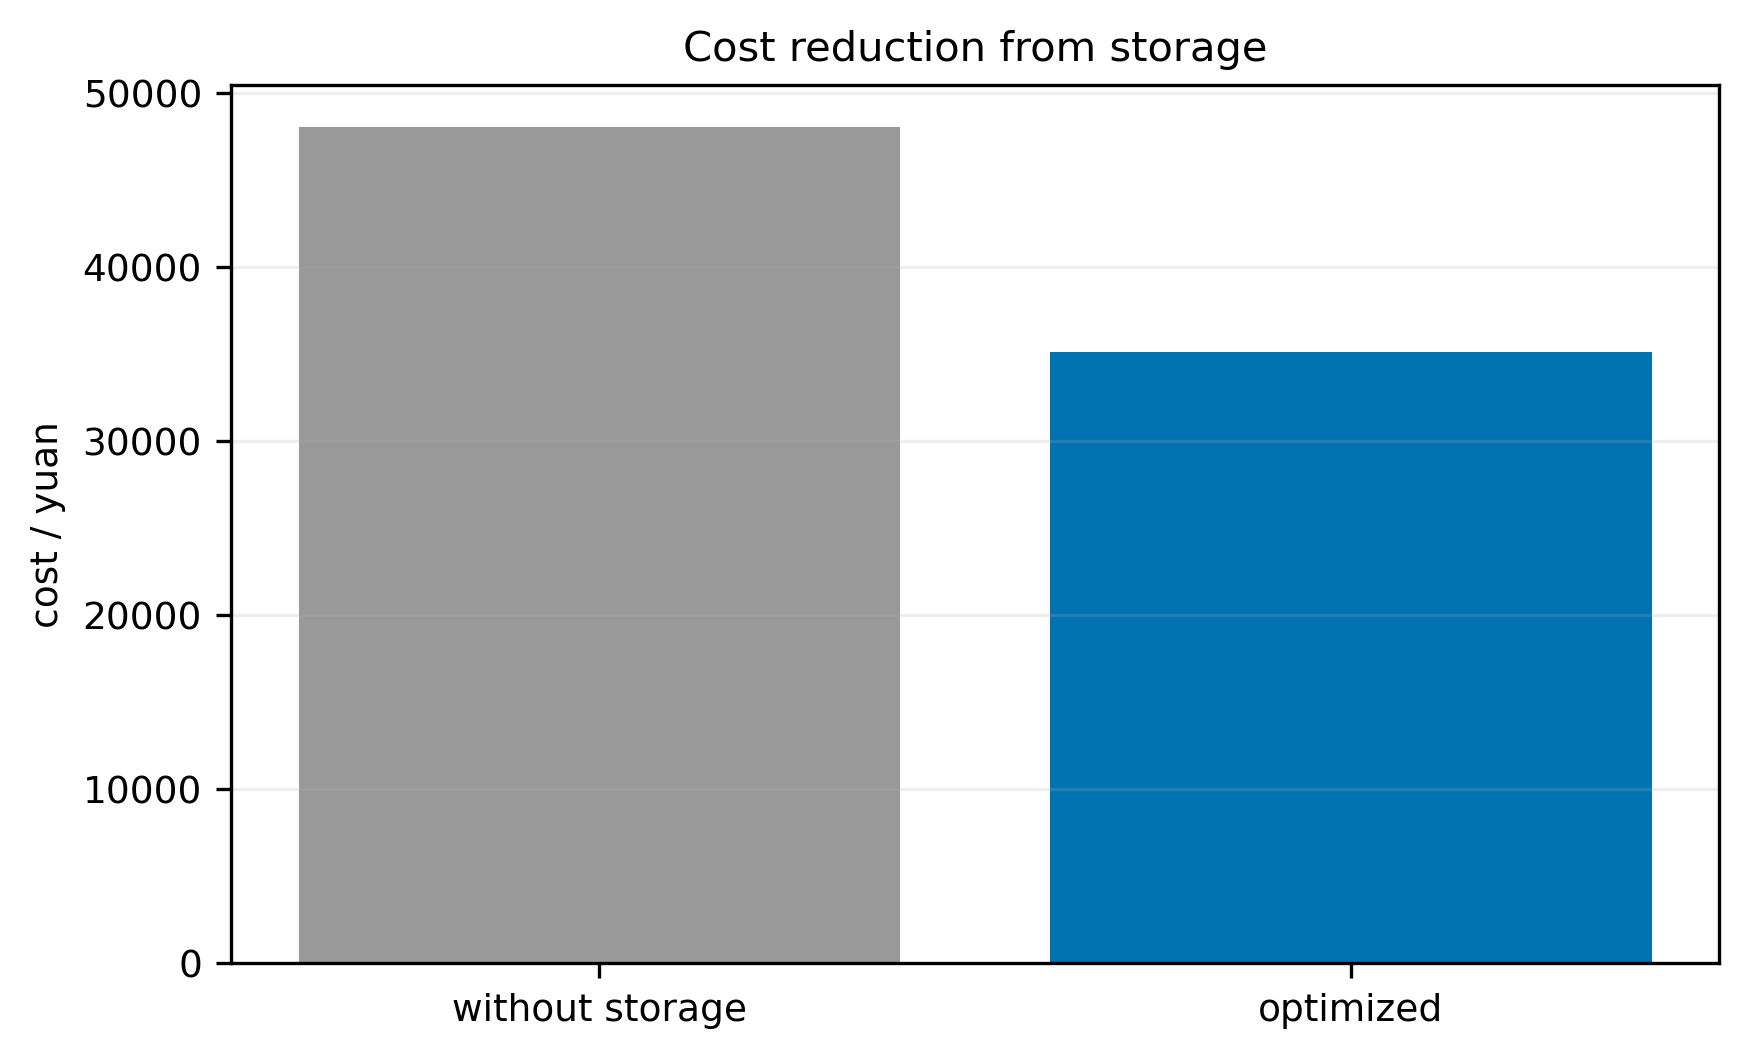
\includegraphics[width=0.72\textwidth]{result_q1_cost.png}
\caption{问题一优化方案与无储能基线的费用对比}
\label{fig:q1-cost}
\end{figure}

结果说明，储能的价值并不是减少总负荷，而是通过时间转移同时利用低价购电和中午光伏富余。由于模型禁止售电，任何额外购电都必须在负荷、充电或状态约束中有明确去向；二阶段吞吐量目标进一步排除了无意义循环。

\section{问题二：含预测误差的全年滚动优化}

\subsection{因果信息集与组合预测}

日前光伏预测具有显著的日内和天气不确定性，模型比较与组合是提高稳定性的常见思路\cite{nespoli2019dayahead,mellit2021deep}。制定第 $d$ 天计划时，本文只允许使用信息集
\begin{equation}
\mathcal F_{d,0}=
\{L_{j,t},P_{j,t}:j<d\}\cup
\{\text{日期、星期和已知固定电价}\}.
\label{eq:q2-info}
\end{equation}
第 $d$ 天的真实负荷、光伏、峰值或由其计算的统计量均不得成为预测特征。

对负荷和光伏分别构造四个基预测器：前一日同刻、前7日同刻均值、前一周同刻以及梯度提升回归。梯度提升方法通过逐步拟合损失函数的负梯度构造加法模型\cite{friedman2001greedy}。每天根据此前最近28天的样本外MAE分配反比权重：
\begin{equation}
\omega_{m,d}=
\frac{(\operatorname{MAE}_{m,d}+\varepsilon)^{-1}}
{\sum_k(\operatorname{MAE}_{k,d}+\varepsilon)^{-1}},
\qquad
\widehat y_{d,t}=\sum_m\omega_{m,d}\widehat y_{d,t}^{(m)}.
\label{eq:q2-ensemble}
\end{equation}
预测结果截断为非负。2月初历史样本较少时，模型自动退化为滞后与滚动统计组合。

采用
\begin{equation}
\operatorname{NMAE}_d=
\frac{\frac1{144}\sum_t|y_{d,t}-\widehat y_{d,t}|}
{\frac1{144}\sum_t|y_{d,t}|}
\label{eq:q2-nmae}
\end{equation}
衡量每日预测误差。334个执行日的负荷、光伏平均NMAE分别为 $5.0016\%$ 和 $7.0387\%$，误差分布见图\ref{fig:q2-forecast-error}。图中保留了全部日观测点，因此少量异常日不会被均值掩盖。

\begin{figure}[H]
\centering
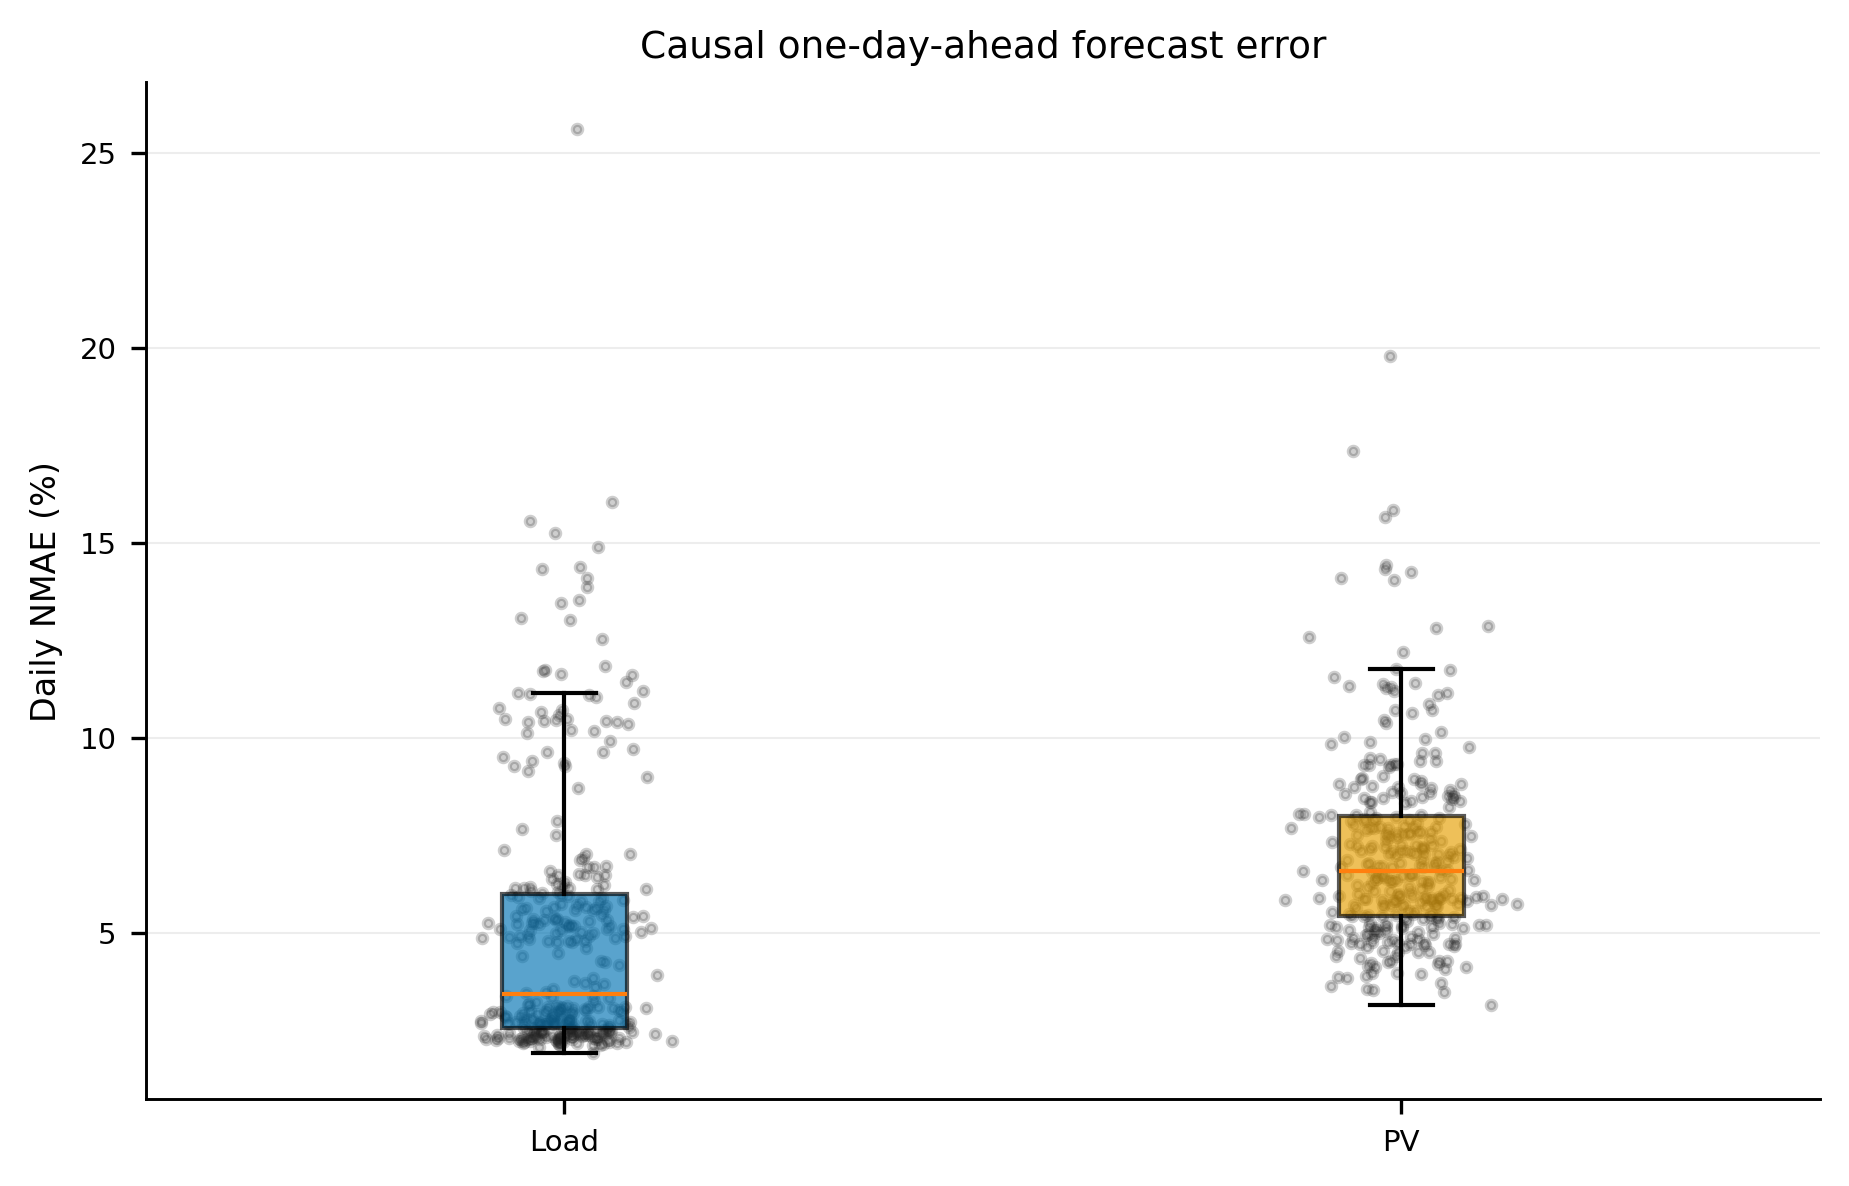
\includegraphics[width=0.84\textwidth]{raw_q2_forecast_error_distribution.png}
\caption{负荷与光伏的因果日前预测误差分布}
\label{fig:q2-forecast-error}
\end{figure}

\subsection{保留日内相关性的残差情景}

定义样本外预测残差向量
\begin{equation}
\bm\varepsilon_j^L=\bm L_j-\widehat{\bm L}_j,\qquad
\bm\varepsilon_j^P=\bm P_j-\widehat{\bm P}_j.
\label{eq:q2-residual}
\end{equation}
在当前执行日前的历史日中抽取整日残差向量，并将两个历史日的残差路径拼接成48小时情景。与逐时段独立抽样相比，该方法保留云层变化、峰荷及相邻时段误差的相关性。第 $s$ 个情景写为
\begin{align}
L_{d,t}^{(s)}&=\max\{0,\widehat L_{d,t}+\varepsilon_{t}^{L,(s)}\},\\
P_{d,t}^{(s)}&=\max\{0,\widehat P_{d,t}+\varepsilon_{t}^{P,(s)}\}.
\label{eq:q2-scenario}
\end{align}
主配置生成30个等概率情景，随机种子固定为20260910。所有残差均来自严格早于执行日的扩展窗口预测，避免用训练拟合残差低估不确定性。

\subsection{48小时两阶段随机MILP}

用随机或鲁棒优化刻画日前市场的不确定性已有相关研究\cite{liu2016bidding}。本文将 $g,c,d,E,z$ 设为全部情景共享的计划变量，将 $h^{(s)},w^{(s)}$ 设为情景结算变量，滚动视窗 $H=\{0,\ldots,287\}$。目标函数为
\begin{equation}
\min\ 
\sum_{t\in H}p_{t\bmod144}g_{d,t}
+\sum_s\pi_s\sum_{t\in H}5p_{t\bmod144}h_{d,t}^{(s)}.
\label{eq:q2-objective}
\end{equation}
第一项是计划购电费，第二项是预测误差情景下的期望紧急购电费。情景能量平衡为
\begin{equation}
g_{d,t}+P_{d,t}^{(s)}\Delta t+d_{d,t}+h_{d,t}^{(s)}
=L_{d,t}^{(s)}\Delta t+c_{d,t}+w_{d,t}^{(s)}.
\label{eq:q2-balance}
\end{equation}

计划储能状态满足
\begin{align}
E_{d,t+1}&=E_{d,t}+\eta_c c_{d,t}-\frac{d_{d,t}}{\eta_d},\\
1200&\le E_{d,t}\le10800,\\
0\le c_{d,t}&\le833.3333z_{d,t},\\
0\le d_{d,t}&\le833.3333(1-z_{d,t}).
\label{eq:q2-storage}
\end{align}
为减弱48小时末端耗尽效应，令 $E_{d,288}=E_{d,0}$。再引入共享二元变量 $y_{d,t}$，规定
\begin{equation}
h_{d,t}^{(s)}\le M_{h,d}y_{d,t},\qquad
c_{d,t}\le833.3333(1-y_{d,t}),
\label{eq:q2-emergency-logic}
\end{equation}
从而任何情景需要紧急购电时，该计划时段不得同时给电池充电。大常数按当天情景负荷动态设置，而非使用固定截断。

\subsection{实际回放与跨日闭环}

滚动优化生成未来48小时计划，但只冻结并执行前144段。计划确定后，才依次读入当天实际负荷与光伏。为保证实际执行满足当前储电量和真实供需，分别将计划放电与充电投影为
\begin{align}
d_{d,t}^{\mathrm{exec}}
&=\min\left\{d_{d,t},\,\eta_d(E_{d,t}^{\mathrm{real}}-E_{\min}),\,
[L_{d,t}^{\mathrm{real}}\Delta t-g_{d,t}-P_{d,t}^{\mathrm{real}}\Delta t]_+\right\},\\
c_{d,t}^{\mathrm{exec}}
&=\min\left\{c_{d,t},\,\frac{E_{\max}-E_{d,t}^{\mathrm{real}}}{\eta_c},\,
[g_{d,t}+P_{d,t}^{\mathrm{real}}\Delta t-L_{d,t}^{\mathrm{real}}\Delta t]_+\right\}.
\label{eq:q2-projection}
\end{align}
紧急购电为
\begin{equation}
h_{d,t}^{\mathrm{real}}=
\left[L_{d,t}^{\mathrm{real}}\Delta t+c_{d,t}^{\mathrm{exec}}
-g_{d,t}-P_{d,t}^{\mathrm{real}}\Delta t-d_{d,t}^{\mathrm{exec}}\right]_+.
\label{eq:q2-real-emergency}
\end{equation}
相应地，实际未利用剩余电量定义为
\begin{equation}
w_{d,t}^{\mathrm{real}}=
\left[g_{d,t}+P_{d,t}^{\mathrm{real}}\Delta t+d_{d,t}^{\mathrm{exec}}
-L_{d,t}^{\mathrm{real}}\Delta t-c_{d,t}^{\mathrm{exec}}\right]_+.
\label{eq:q2-real-surplus}
\end{equation}
于是每个时段满足完整的实际能量平衡与缺口、剩余互补关系
\begin{equation}
g_{d,t}+P_{d,t}^{\mathrm{real}}\Delta t+d_{d,t}^{\mathrm{exec}}+h_{d,t}^{\mathrm{real}}
=L_{d,t}^{\mathrm{real}}\Delta t+c_{d,t}^{\mathrm{exec}}+w_{d,t}^{\mathrm{real}},
\qquad h_{d,t}^{\mathrm{real}}w_{d,t}^{\mathrm{real}}=0.
\label{eq:q2-real-balance}
\end{equation}
日末实际状态通过
\begin{equation}
E_{d,t+1}^{\mathrm{real}}=
E_{d,t}^{\mathrm{real}}+\eta_c c_{d,t}^{\mathrm{exec}}
-\frac{d_{d,t}^{\mathrm{exec}}}{\eta_d},
\qquad
E_{d+1,0}^{\mathrm{real}}=E_{d,144}^{\mathrm{real}}
\label{eq:q2-real-state}
\end{equation}
传给次日；状态链起点采用前述 $E_{d_0,0}^{\mathrm{real}}=6000$ kWh。由此，预测误差影响的是当天计划质量和当天费用，而不是作为虚假的预测状态被全年继承。使用实际值结算并非事后修改计划，因为 $g_{d,t}$ 在当天0:00已经冻结。

\subsection{求解限时与回退机制}

单日首先求解30情景模型；达到时间限制而未获得满足门限的解时，依次回退为10情景模型和Q80确定性模型。Q80来自单时段报童问题的分位数解释：当计划电量单价为 $p_t$、缺口惩罚为 $5p_t$ 时，不计储能耦合的临界分位数满足
\begin{equation}
\Pr(N_t\le q_t^\star)=1-\frac{p_t}{5p_t}=0.8.
\label{eq:q2-q80}
\end{equation}
因此Q80可作为保守且有经济含义的最后回退，而不是任意常数。

图\ref{fig:q2-modes}给出全年实际采用的模式：30情景主模型62天、10情景回退271天、Q80回退1天。Q80回退发生在2025年4月8日。该分布说明在给定计算时限下，全年结果是混合执行策略，不能表述为纯30情景方案。

\begin{figure}[H]
\centering
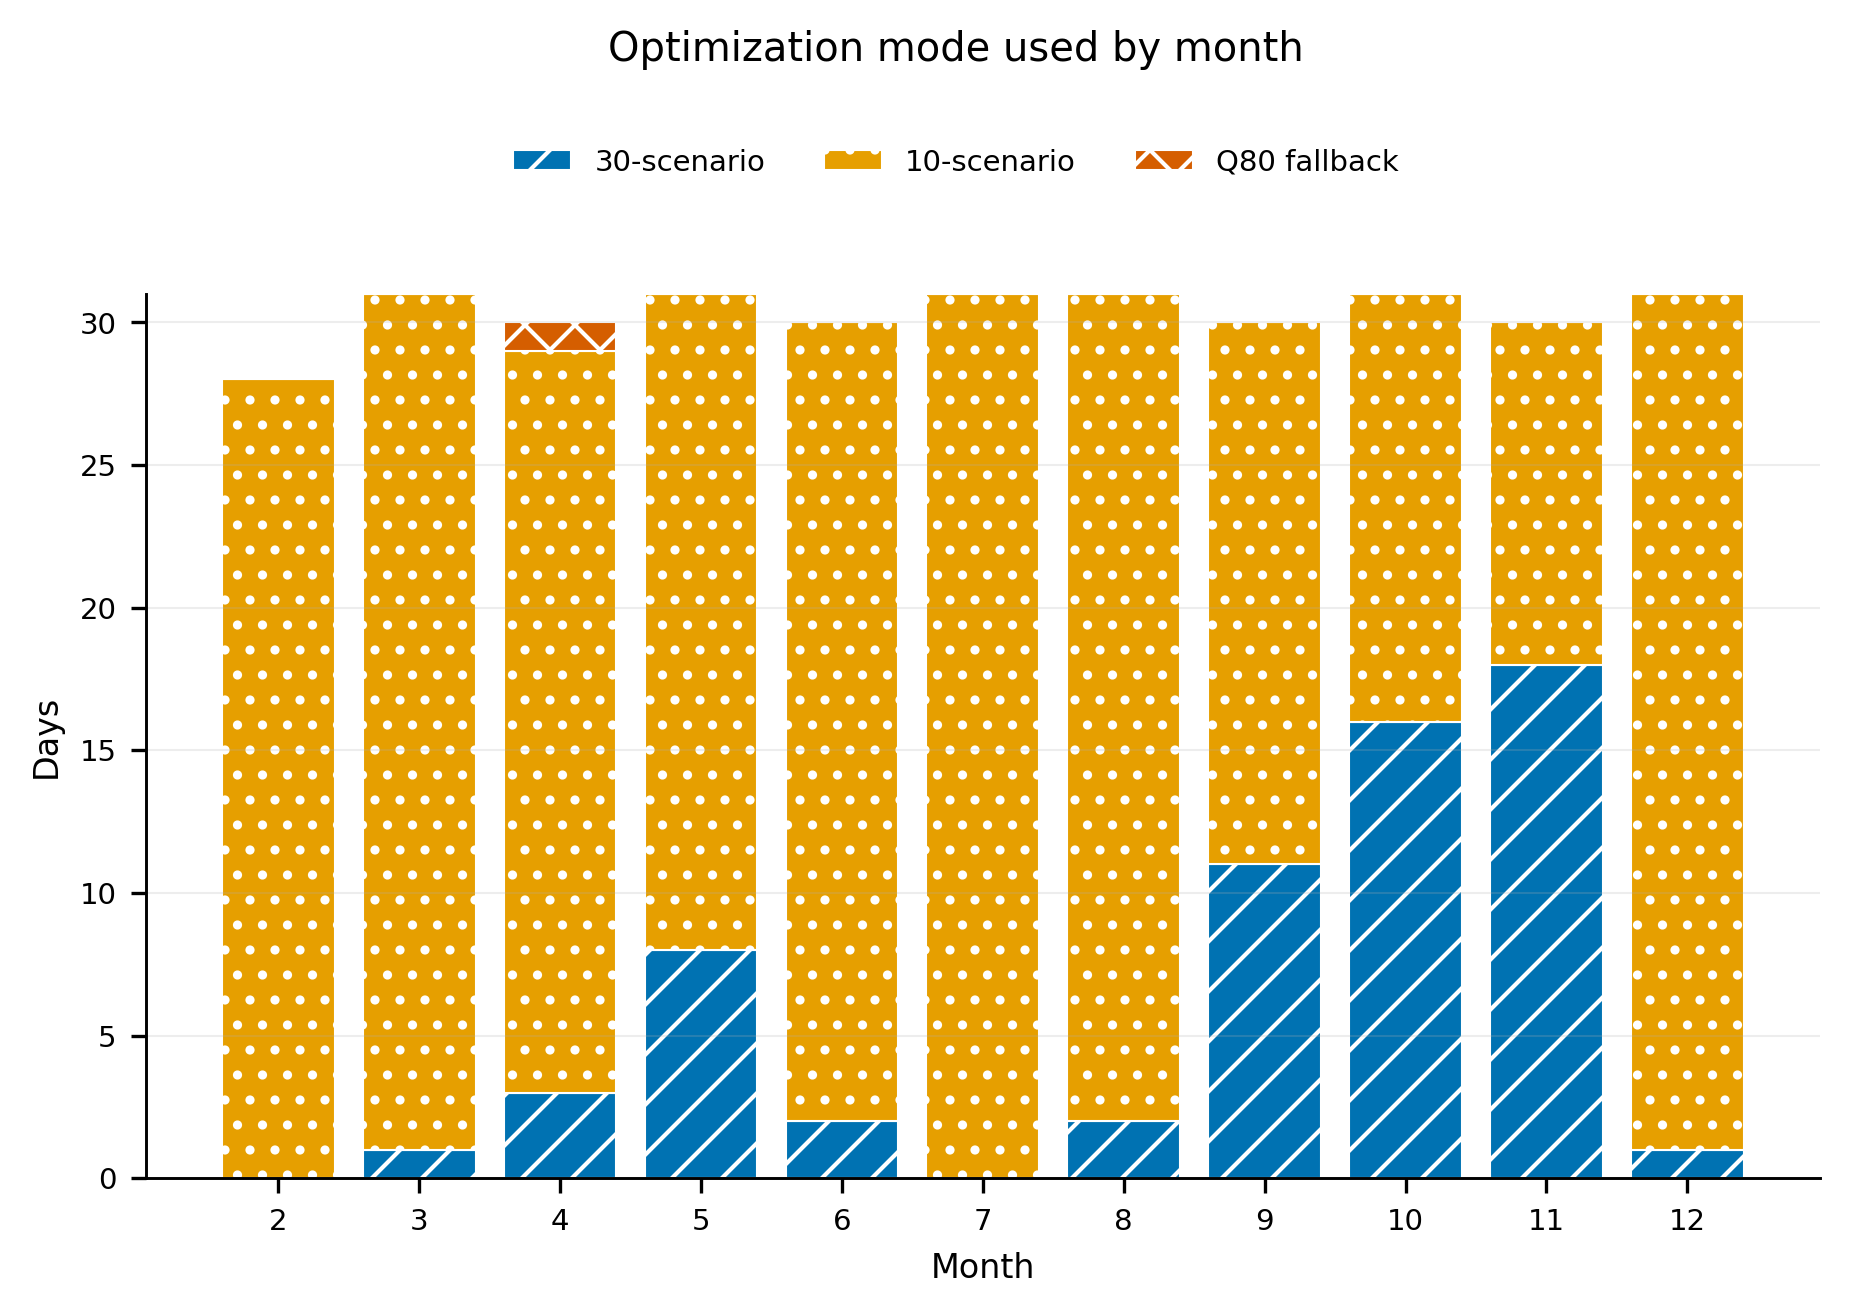
\includegraphics[width=0.86\textwidth]{process_q2_solver_modes.png}
\caption{全年各月实际采用的优化模式}
\label{fig:q2-modes}
\end{figure}

\subsection{全年结果}

实际日总费用为
\begin{equation}
C_d^{\mathrm{real}}=
\sum_{t=0}^{143}p_tg_{d,t}
+\sum_{t=0}^{143}5p_th_{d,t}^{\mathrm{real}}.
\label{eq:q2-real-cost}
\end{equation}
表\ref{tab:q2-summary}汇总2025年2月1日至12月31日的回放结果。计划购电费占总费用的 $91.41\%$，紧急购电费占 $8.59\%$。

\begin{table}[H]
\centering
\caption{问题二全年总体结果}
\label{tab:q2-summary}
\begin{tabular}{lr}
\toprule
指标 & 数值\\
\midrule
执行天数 & 334\\
10分钟时段数 & 48096\\
计划购电费用/元 & 13670139.413005\\
紧急购电费用/元 & 1284715.793694\\
总费用/元 & 14954855.206699\\
紧急购电量/kWh & 301509.748286\\
未利用剩余电量/kWh & 3638778.813938\\
负荷平均日NMAE & 5.0016\%\\
光伏平均日NMAE & 7.0387\%\\
平均日总费用/元 & 44775.015589\\
\bottomrule
\end{tabular}
\end{table}

图\ref{fig:q2-storage}显示实际日初与日末储电量在全年连续传递，两条曲线相邻日首尾重合。储电量始终位于 $[1200,10800]$ kWh。该图直接验证了“继承实际状态而非预测状态”的闭环机制。

\begin{figure}[H]
\centering
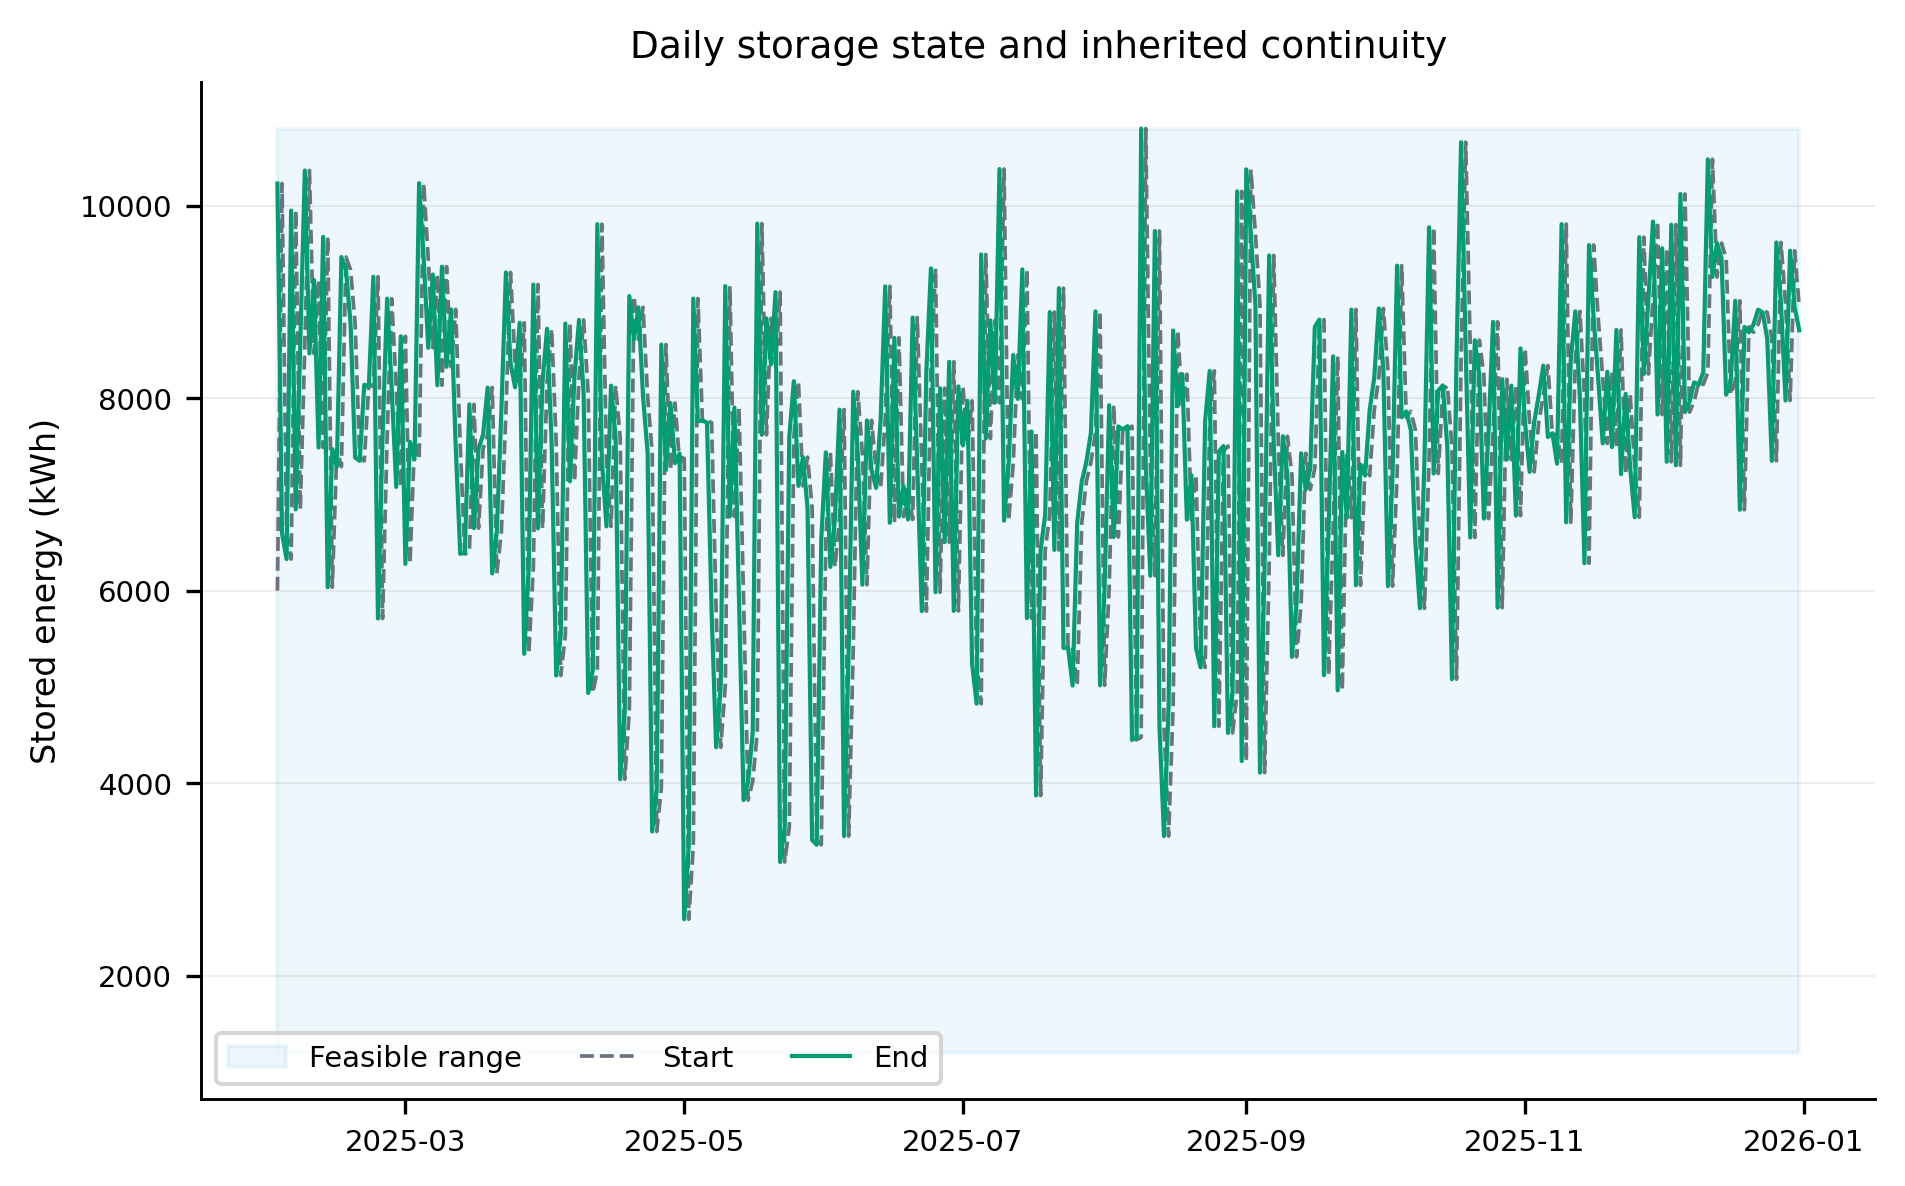
\includegraphics[width=0.94\textwidth]{process_q2_storage_state.png}
\caption{全年实际储能状态及跨日连续性}
\label{fig:q2-storage}
\end{figure}

月度费用分解如图\ref{fig:q2-month-cost}所示，12月总费用最高，4月最低；6月和7月的紧急购电附加费用相对突出。月度数值见表\ref{tab:q2-monthly}。

\begin{figure}[H]
\centering
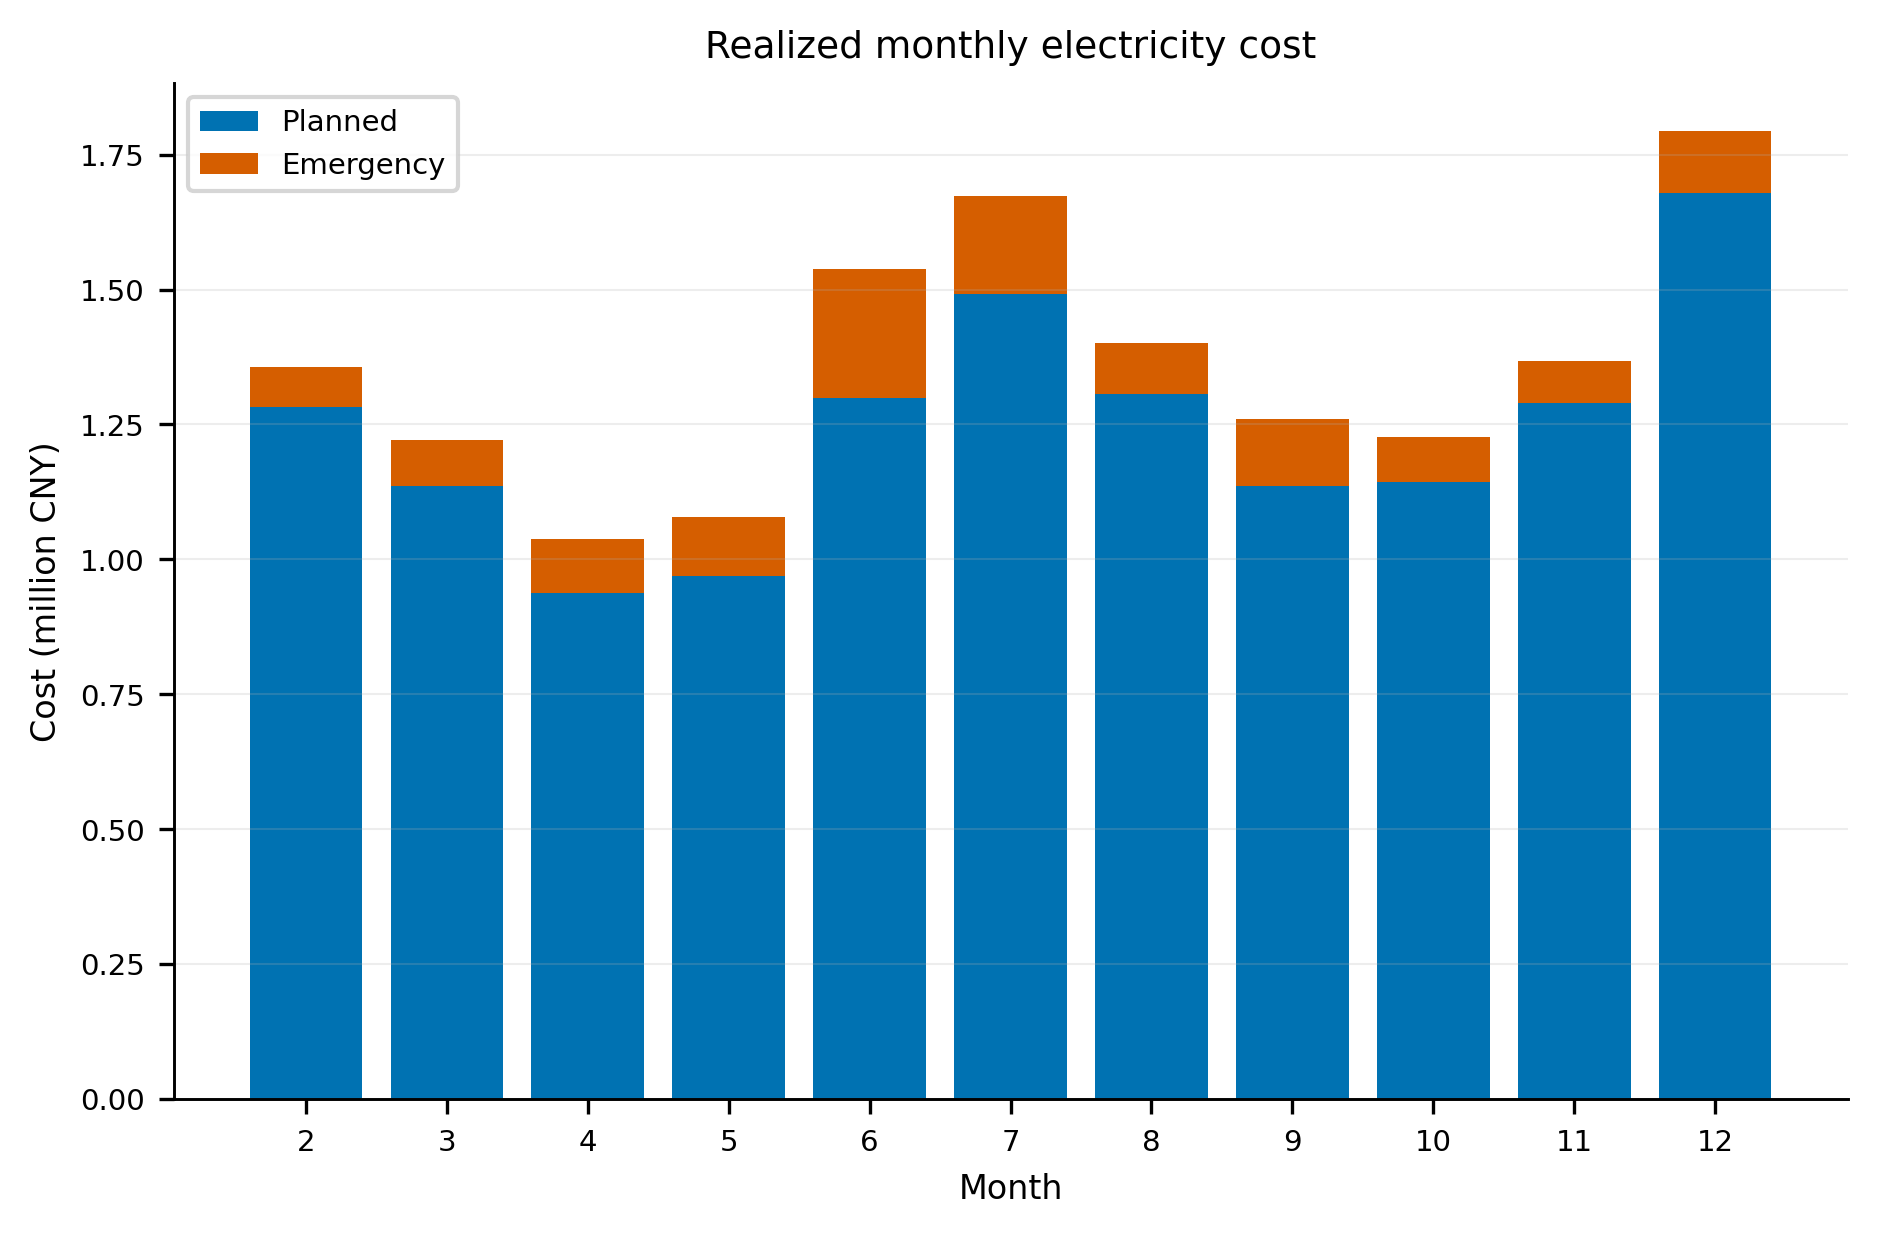
\includegraphics[width=0.86\textwidth]{result_q2_monthly_cost.png}
\caption{全年各月计划购电费与紧急购电费}
\label{fig:q2-month-cost}
\end{figure}

\begin{table}[H]
\centering
\caption{问题二月度费用与紧急购电量}
\label{tab:q2-monthly}
\small
\begin{tabular}{crrr}
\toprule
月份 & 计划费用/万元 & 紧急费用/万元 & 紧急购电量/MWh\\
\midrule
2月 & 128.3014 & 7.3600 & 16.8399\\
3月 & 113.5324 & 8.5859 & 21.1129\\
4月 & 93.8594 & 9.9646 & 23.0255\\
5月 & 96.9594 & 10.8354 & 25.2593\\
6月 & 129.9354 & 23.9131 & 53.4436\\
7月 & 149.1003 & 18.2379 & 43.9601\\
8月 & 130.5890 & 9.5109 & 22.1721\\
9月 & 113.5394 & 12.5580 & 27.8633\\
10月 & 114.3103 & 8.3118 & 19.3326\\
11月 & 128.9724 & 7.7677 & 18.5532\\
12月 & 167.9146 & 11.4261 & 29.9474\\
\bottomrule
\end{tabular}
\end{table}

\subsection{指定日期计划}

题目模板要求重点展示2025年2月1日、5月1日、8月1日和11月1日。图\ref{fig:q2-days}给出这4天的计划购电功率等效值与实际紧急购电。2月1日未出现紧急购电；5月1日多个时段发生小规模紧急购电；8月1日和11月1日只出现少量尖峰。图中计划购电的分段变化来自电价、预测净负荷和储能边界的共同作用。

\begin{figure}[H]
\centering
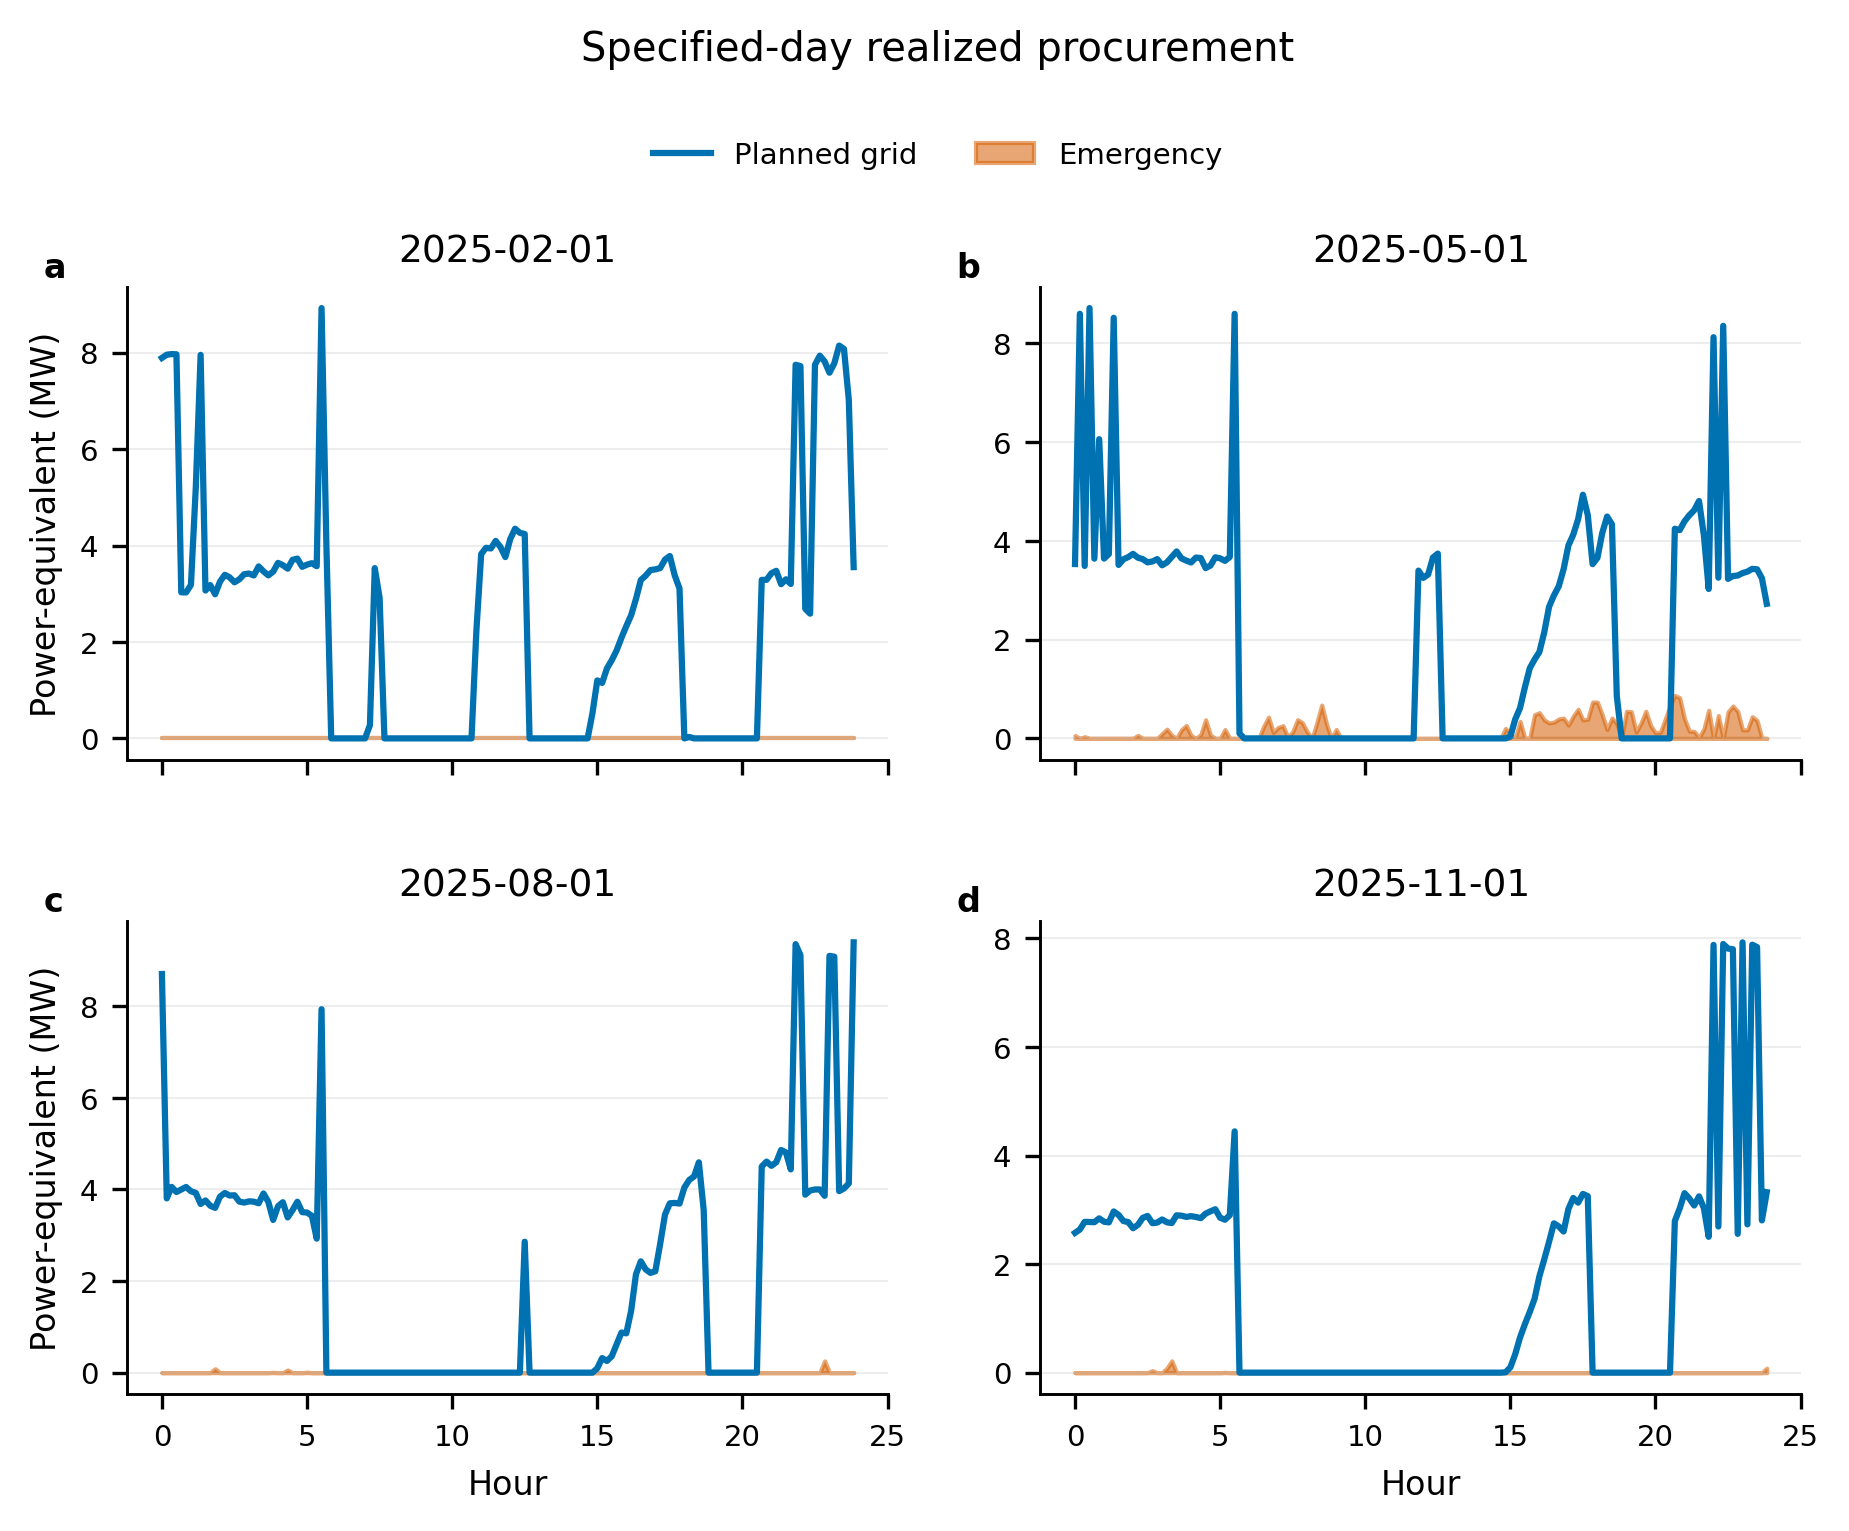
\includegraphics[width=0.96\textwidth]{result_q2_specified_dates.png}
\caption{四个指定日期的计划购电与实际紧急购电}
\label{fig:q2-days}
\end{figure}

\subsection{日末储能价值的备选实验}

现有48小时模型通过后24小时预测及视窗末循环约束表达未来影响，并未要求每天24:00恢复到6000 kWh。作为备选，若只建立24小时模型，可在目标中加入日末储能价值
\begin{equation}
\min\left\{
\sum_{t=0}^{143}p_tg_{d,t}
+\sum_s\pi_s\sum_{t=0}^{143}5p_th_{d,t}^{(s)}
-v_dE_{d,144}\right\}.
\label{eq:q2-terminal-value}
\end{equation}
其中 $v_d$ 必须在当天0:00用已知信息估计。本文用当时已生成的次日预测，在储电量相差 $\Delta E=100$ kWh 的两个初值下求解次日问题，取
\begin{equation}
v_d\approx
\frac{J_{d+1}^{*}(E)-J_{d+1}^{*}(E+\Delta E)}{\Delta E},
\label{eq:q2-terminal-fd}
\end{equation}
且不读取次日真实数据。

为检验该思路，选取2月、5月、8月和11月各连续14天，共56天；每个窗口内各策略从相同实际储电量出发并连续继承自身状态。所有24小时实验分支使用相同的因果预测、10条残差情景、种子和求解门限，$v=0$ 是严格受控基线。表\ref{tab:q2-terminal-value}显示，动态 $v_d$ 的均值为0.4619元/kWh，相对基线使实际费用减少385.49元、紧急费用减少1985.52元，并在四个截断窗口末合计多保留5986.32 kWh。以0.45元/kWh统一折算截断窗口末库存后，差额为 $-3079.33$ 元。

\begin{table}[H]
\centering
\caption{24小时终端价值受控实验（四个14天窗口）}
\label{tab:q2-terminal-value}
\small
\begin{tabular}{lrrrrr}
\toprule
策略 & 实际费用差/元 & 紧急费用差/元 & 末库存差/kWh & 折算差/元 & 触及上限/天\\
\midrule
动态 $v_d$ & -385.49 & -1985.52 & 5986.32 & -3079.33 & 1\\
$v=0$ & 0 & 0 & 0 & 0 & 0\\
$v=0.3$ & 113.76 & 6.48 & 0 & 113.76 & 0\\
$v=0.5$ & 30372.33 & -7179.63 & 34723.07 & 14746.95 & 37\\
$v=0.8$ & 35250.09 & -7439.11 & 34948.89 & 19523.09 & 49\\
$v=1.0$ & 35297.54 & -7395.57 & 34948.89 & 19570.54 & 49\\
\bottomrule
\end{tabular}
\end{table}

固定 $v\ge0.5$ 虽降低部分紧急费用，却在37--49天把日末储电量推至10800 kWh上限，并因额外购电和弃能使总费用上升。这说明固定线性价值容易产生阈值型的“全保留”决策；动态 $v_d$ 或分段线性价值函数 $V_d(E)$ 更合理。不过该实验只覆盖56天，不能替代现有334天正式结果；若切换主方案，还需在同一配置下完成全年A/B测试并统一处理12月31日末端库存。

\section{问题三：每6小时再调度与预测窗口比较}

\subsection{滚动承诺与调整成本}

问题三在每天0:00、6:00、12:00和18:00共进行4次决策。记第 $k$ 次发布后对尚未执行时段 $t$ 的有效购电承诺为 $g_{d,t}^{(k)}$。在0:00形成全天基准计划，其费用为
\begin{equation}
C_d^{\mathrm{base}}=\sum_{t=0}^{143}p_tg_{d,t}^{(0)}.
\end{equation}
对于 $k>0$ 的再调度，令 $u_{d,t}^{(k)}$、$v_{d,t}^{(k)}$ 分别表示增购和退购，则
\begin{equation}
g_{d,t}^{(k)}-g_{d,t}^{(k-1)}=u_{d,t}^{(k)}-v_{d,t}^{(k)},\qquad u_{d,t}^{(k)},v_{d,t}^{(k)}\ge0.
\end{equation}
相应调整费用直接进入优化目标：
\begin{equation}
C_d^{\mathrm{adj}}=\sum_{k=1}^{3}\sum_{t\in\mathcal T_k}
\left(1.5p_tu_{d,t}^{(k)}-0.5p_tv_{d,t}^{(k)}\right),
\end{equation}
其中 $\mathcal T_k$ 是第 $k$ 次发布时尚未执行的当日时段。这样，优化器会同时衡量新增承诺的成本与退购返还，而不会把调整视为事后免费修正。图~\ref{fig:q3-adjust}显示两种窗口在4个发布时刻的平均上调和退购规模。

\begin{figure}[H]
\centering

\includegraphics[width=0.86\textwidth]{process_q3_adjustment_epochs.png}
\caption{H24与H48在各发布时刻的平均购电调整量}
\label{fig:q3-adjust}
\end{figure}

\subsection{统一的预测窗口模型}

两种方案只在预测长度上不同：H24取 $T_H=144$，H48取 $T_H=288$。每次发布均根据当时可得的历史负荷、历史预测残差和附件3光伏预报构造场景；当天真实负荷和光伏仍只用于发布后的回放。对场景 $s$ 和窗口内时段 $t$，能量平衡为
\begin{equation}
g_t+P_t^{(s)}\Delta t+d_t+h_t^{(s)}
=L_t^{(s)}\Delta t+c_t+w_t^{(s)}.
\end{equation}
储能递推及互斥约束为
\begin{align}
E_{t+1}&=E_t+\eta_cc_t-\frac{d_t}{\eta_d},\\
E_{\min}&\le E_t\le E_{\max},\\
0\le c_t&\le Q_{\max}z_t,\qquad
0\le d_t\le Q_{\max}(1-z_t).
\end{align}
为避免较短窗口在末端无代价放空电池，两方案均采用同一循环末端条件
\begin{equation}
E_{T_H}=E_0.
\end{equation}
该约束只作用于每次规划中的预测状态；实际状态仍由前6小时的真实回放形成，并传入下一次更新。因此，H48的潜在优势来自能够看到次日价格、负荷和光伏结构，从而提前安排储能，而不是来自不同的终端规则。

\subsection{锁定执行与实际回放}

每次优化完成后仅锁定前36个十分钟时段。对锁定区间，使用实际负荷与光伏依次执行“有效购电承诺+光伏+储能调节”；若仍有缺口，再以5倍电价紧急购电。第 $d$ 日总费用为
\begin{equation}
C_d=C_d^{\mathrm{base}}+C_d^{\mathrm{adj}}
+\sum_{t=0}^{143}5p_th_{d,t}^{\mathrm{real}}.
\end{equation}
实际日末状态连续传递：
\begin{equation}
E_{d+1,0}=E_{d,144}^{\mathrm{real}}.
\end{equation}
H24与H48在同一日期、同一发布时刻使用相同残差样本日和相同场景数；只要任一方案在某一场景级别失败，就同时丢弃两者并在较低场景级别从头运行，避免不对称回退造成偏差。

\subsection{全年配对实验结果}

正式实验覆盖2025年2月1日至12月31日，共334天。每次优化采用10条历史整段残差情景，并将单次MILP求解上限设为120秒；H24与H48均由主模型完成，未发生确定性回退。两种视窗在相同发布时刻共享情景编号和概率，以保证配对公平。全年汇总见表~\ref{tab:q3summary}。

\begin{table}[H]
\centering
\caption{问题三两种预测窗口的全年配对结果}
\label{tab:q3summary}
\begin{tabular}{lrr}
\toprule
指标 & H24 & H48\\
\midrule
总费用/元 & 15464289.45 & 15358936.78\\
0:00基准计划费用/元 & 14367086.55 & 14246007.21\\
调整费用/元 & 360721.66 & 387387.28\\
紧急购电费用/元 & 736481.23 & 725542.29\\
紧急购电量/kWh & 187401.26 & 184302.63\\
紧急购电时段数 & 6498 & 6430\\
平均日末储电量/kWh & 10561.38 & 7469.00\\
最低日末储电量/kWh & 7688.43 & 2816.82\\
求解总耗时/s & 389.66 & 2901.43\\
\bottomrule
\end{tabular}
\end{table}

H48总费用比H24低 $105352.66$ 元，降幅约 $0.681\%$。它的调整费用多 $26665.62$ 元，但0:00基准计划费用和紧急购电费用分别少 $121079.34$ 元和 $10938.94$ 元，抵消了额外调整成本。图~\ref{fig:q3-cost}直观展示这一分项关系。

\begin{figure}[H]
\centering

\includegraphics[width=0.70\textwidth]{result_q3_cost_components.png}
\caption{H24与H48全年费用分项比较}
\label{fig:q3-cost}
\end{figure}

逐日配对差定义为 $D_d=C_d^{\mathrm{H24}}-C_d^{\mathrm{H48}}$。为保留日序列相关性，采用7日循环移动块bootstrap，重复5000次。日均差的95\%置信区间为 $[258.87,371.89]$ 元/日，完全大于0。图~\ref{fig:q3-cum}显示累计差虽在个别日期短暂波动，但全年总体向正方向增长。

\begin{figure}[H]
\centering

\includegraphics[width=0.88\textwidth]{result_q3_cumulative_cost_difference.png}
\caption{全年累计费用差 $\sum_d(C_d^{\mathrm{H24}}-C_d^{\mathrm{H48}})$}
\label{fig:q3-cum}
\end{figure}

\subsection{指定日期与机制解释}

题目指定的3月20日、6月21日和12月21日，H48分别节省683.13、662.68和195.29元；9月23日H48反而多支出624.78元。图~\ref{fig:q3-storage}给出这4天的实际储能轨迹。H24的日末储能多次接近上限，而H48利用次日信息更积极地释放和补充储能；这与其较低的全年基准费用一致。但H48求解总耗时约为H24的7.45倍，若硬件或时间更紧，应把H24作为快速备选。

\begin{figure}[H]
\centering

\includegraphics[width=0.90\textwidth]{process_q3_storage_specified.png}
\caption{4个指定日期的H24与H48实际储能轨迹}
\label{fig:q3-storage}
\end{figure}

综合费用、紧急购电和置信区间，在当前10情景设定下推荐H48。由于尚未完成不同场景数和终端条件的统一全年敏感性实验，该推荐只对本文计算设置成立。

\section{问题四：波动电价下的因果滚动调度}

\subsection{电价预测与信息边界}

附件4给出2025年365天、每日144个时段的实际电价。其价格范围为 $0.0076$--$1.7936$ 元/kWh，均值为 $0.7662$ 元/kWh，标准差为 $0.3407$ 元/kWh；相邻10分钟价格相关系数为 $0.9641$，说明电价既有明显日内连续性，也存在跨日变化。为避免使用未来真实价格，计划阶段对目标日 $d'$ 的第 $t$ 个时段采用周滞后预测
\begin{equation}
\widehat p_{d',t}=p^{\mathrm{real}}_{d'-7,t}.
\end{equation}
当48小时窗口跨越次日时，对窗口中每个目标日分别取其7日前同一时段价格。因此，第 $d$ 日计划只使用不晚于 $d-1$ 日的数据；附件4目标时段真实价格仅在计划冻结后进入回放结算。负荷与光伏仍沿用问题三的10条历史整段残差情景。

\subsection{波动电价目标函数与执行规则}

计划优化沿用问题三的储能状态、功率平衡、充放电互斥和终端状态约束，只把固定价格序列替换为预测价格。设当前发布时刻为 $k$，基准承诺为 $g_{d,t}^{(0)}$，则计划目标中的购电与调整费用为
\begin{equation}
\sum_t \widehat p_{d,t}g_{d,t}^{(0)}+
\sum_{k=1}^{3}\sum_t\left(1.5\widehat p_{d,t}u_{d,t}^{(k)}-0.5\widehat p_{d,t}v_{d,t}^{(k)}\right),
\end{equation}
并叠加各负荷--光伏情景下的期望紧急购电费用。计划锁定后，所有费用改用目标时段的真实价格结算：
\begin{equation}
C_d=\sum_t p^{\mathrm{real}}_{d,t}g_{d,t}^{(0)}+
\sum_{k,t}\left(1.5p^{\mathrm{real}}_{d,t}u_{d,t}^{(k)}-0.5p^{\mathrm{real}}_{d,t}v_{d,t}^{(k)}\right)
+\sum_t5p^{\mathrm{real}}_{d,t}h_{d,t}^{\mathrm{real}}.
\end{equation}
问题4-2仅在每日0:00优化并执行全天，不产生日内调整费用；问题4-3在0:00、6:00、12:00和18:00更新，每次只执行前6小时。两问均比较H24与H48视窗，实际日末储电量连续传递至下一天。

\subsection{全年实验结果}

实验覆盖2025年2月1日至12月31日，共334天。每次求解采用10条负荷--光伏情景，单次时限60秒，全部由主模型完成，无回退事件。问题4-2结果见表~\ref{tab:q42summary}。

\begin{table}[H]
\centering
\caption{问题4-2每日决策下的全年结果}
\label{tab:q42summary}
\begin{tabular}{lrr}
\toprule
指标 & H24 & H48\\
\midrule
总费用/元 & 16548003.63 & 16338121.68\\
基准购电费用/元 & 15066465.38 & 14851331.00\\
紧急购电费用/元 & 1481538.24 & 1486790.68\\
紧急购电量/kWh & 311791.12 & 315920.39\\
紧急购电时段数 & 7963 & 8136\\
平均日末储电量/kWh & 10742.31 & 5407.91\\
最低日末储电量/kWh & 8663.27 & 1200.00\\
求解总耗时/s & 111.45 & 736.00\\
\bottomrule
\end{tabular}
\end{table}

问题4-2中H48比H24节省 $209881.95$ 元，降幅为 $1.268\%$。H48的紧急购电费略高 $5252.43$ 元，但基准购电费降低 $215134.38$ 元，说明48小时视窗的主要收益来自跨日电价套利与储能配置，而不是减少供能缺口。逐日费用差的7日移动块bootstrap 95\%置信区间为 $[500.96,760.31]$ 元/日。

问题4-3结果见表~\ref{tab:q43summary}。日内再调度明显降低了两种视窗的紧急购电费用和总费用。

\begin{table}[H]
\centering
\caption{问题4-3每6小时再调度下的全年结果}
\label{tab:q43summary}
\begin{tabular}{lrr}
\toprule
指标 & H24 & H48\\
\midrule
总费用/元 & 16245477.76 & 16080198.49\\
基准购电费用/元 & 15059188.53 & 14865588.55\\
调整费用/元 & 415968.93 & 456819.71\\
紧急购电费用/元 & 770320.30 & 757790.23\\
紧急购电量/kWh & 181777.13 & 177604.73\\
紧急购电时段数 & 6316 & 6249\\
平均日末储电量/kWh & 10557.48 & 5305.70\\
最低日末储电量/kWh & 7809.37 & 1200.00\\
求解总耗时/s & 654.17 & 1949.18\\
\bottomrule
\end{tabular}
\end{table}

问题4-3中H48比H24节省 $165279.28$ 元，降幅为 $1.017\%$，逐日费用差95\%置信区间为 $[401.90,588.93]$ 元/日。与问题4-2相比，H24和H48分别再节省 $302525.87$ 元和 $257923.19$ 元，表明6小时更新能够利用最新负荷、光伏信息修正计划。图~\ref{fig:q4-cost}汇总了两种执行规则与两种视窗的费用关系。综合成本与稳定性，问题四仍推荐H48；若更重视求解速度，则H24为可行备选。

\begin{figure}[H]
\centering

\includegraphics[width=0.72\textwidth]{result_q4_total_cost_comparison.png}
\caption{波动电价下每日决策与6小时再调度的全年总费用}
\label{fig:q4-cost}
\end{figure}

\section{模型验证与结果可信度}

\subsection{数值与物理约束验证}

对逐时结果独立复算能量平衡、储能递推、跨日连续性和费用。表\ref{tab:validation}显示，实际层残差达到浮点误差量级；计划层与情景层残差远小于单时段数百kWh的能量规模。所有状态均满足闭区间边界，且实际执行层未出现紧急购电与充电同时发生。问题三和问题四在情景计划层出现少量紧急购电与充电或弃电同时为正的记录，数值位于MILP容差附近，故自动验证报告从严标记为未全部通过；这些记录不影响实际执行层的功率平衡，但正式结论保留该限制。

\begin{table}[H]
\centering
\caption{四问数值与逻辑验证}
\label{tab:validation}
\begin{tabular}{p{8.2cm}r}
\toprule
验证指标 & 数值\\
\midrule
问题一最大能量平衡残差/kWh & $2.27\times10^{-13}$\\
问题一最大状态递推残差/kWh & $8.31\times10^{-13}$\\
问题一同时充放电时段数 & 0\\
问题二最大实际能量平衡残差/kWh & $5.68\times10^{-13}$\\
问题二最大实际状态递推残差/kWh & $5.46\times10^{-12}$\\
问题二最大跨日状态缺口/kWh & 0\\
问题二最大计划状态残差/kWh & $1.19\times10^{-7}$\\
问题二最大情景平衡残差/kWh & $1.48\times10^{-7}$\\
问题二实际储电量范围/kWh & $[1200,10800]$\\
问题二计划同时充放电时段数 & 0\\
问题三逐时段/每日/更新级记录数 & $96192/668/2672$\\
问题三最大实际平衡残差/kWh & $2.27\times10^{-13}$\\
问题三最大实际状态残差/kWh & $9.09\times10^{-13}$\\
问题三最大计划/场景平衡残差/kWh & $8.20\times10^{-8}/1.16\times10^{-7}$\\
问题三最大MILP gap & $9.99\times10^{-7}$\\
问题三计划层紧急充电/紧急弃电计数 & $8/2$\\
问题4-2最大实际平衡/状态残差/kWh & $2.27\times10^{-13}/9.09\times10^{-13}$\\
问题4-2最大计划/场景平衡残差/kWh & $1.30\times10^{-8}/2.18\times10^{-9}$\\
问题4-2计划层紧急充电/紧急弃电计数 & $1/0$\\
问题4-3最大实际平衡/状态残差/kWh & $2.27\times10^{-13}/9.09\times10^{-13}$\\
问题4-3最大计划/场景平衡残差/kWh & $1.91\times10^{-8}/6.69\times10^{-9}$\\
问题4-3计划层紧急充电/紧急弃电计数 & $12/3$\\
\bottomrule
\end{tabular}
\end{table}

\subsection{因果性验证}

全年共有668条预测指标，即334个执行日分别对应负荷和光伏。每条记录的训练截止日均为执行日前一天；每个执行日抽取的历史残差日期严格早于执行日。预测阶段不读取当日真实值，实际值只在计划冻结后进入回放。因此，本文报告的是样本外滚动执行费用，而不是把全年真实曲线预先交给优化器得到的事后最优费用。

问题三的2672条更新记录均保存训练截止日、发布时刻、抽样残差日和求解模式。H24与H48在每个配对更新点的求解模式、场景数和样本日完全一致。6:00、12:00和18:00发布计划时，已经发生区间的真实负荷与光伏可用于因果偏差修正；尚未发生区间的真实值只能在计划发布后进入回放。由此可排除方案间信息集不一致或未来数据泄漏导致的虚假优势。

问题四的价格预测对每个目标时段只调用7日前同刻价格；真实波动电价仅在计划冻结后的结算表达式中读取。问题4-2与问题4-3分别生成668条和2672条更新级记录，H24与H48在同一更新点保持相同场景数和负荷--光伏样本路径。因此，第四问结果也是因果回放结果，而非已知全年价格后的事后最优解。

\subsection{费用与模板复算}

计划费用通过 $\sum p_tg_{d,t}$ 逐时复算为 $13670139.413004687$ 元，紧急费用通过 $\sum5p_th_{d,t}^{\mathrm{real}}$ 复算为 $1284715.793694495$ 元，与每日汇总完全一致。结果工作簿包含334行计划购电、2004行六段充放电汇总和3591行紧急购电模板数据，其中3570行为正紧急购电区间、21行为无紧急购电日期的零值占位；日期、144个时段表头及四个指定日期均与CSV一致。

问题三结果工作簿采用H48方案：计划购电量表写0:00基准计划，调整购电量表写三次滚动修正后的最终有效承诺，全天费用写基准费用与净调整费用之和。工作簿包含334行计划、334行调整、2004行六段充放电记录和2992条紧急购电记录，其中2985条为正紧急购电区间，7条为无紧急购电日期的“无”和0占位。逐时段CSV另保存最终承诺减基准计划的净调整量，便于复算调整恒等式。

问题4-2和问题4-3分别生成96192条逐时记录，均等于 $334\times144\times2$。其每日汇总中的总费用与“真实价格基准费用+真实价格调整费用+5倍真实价格紧急费用”逐项求和一致；两问的H24--H48总费用差分别复算为 $209881.95$ 元和 $165279.28$ 元。完整逐时数据、每日指标、更新级验证与复现清单分别保存在两套正式结果目录中。

\section{模型评价与适用边界}

\subsection{模型优点}

\begin{enumerate}
  \item \textbf{量纲和物理约束明确。} 功率统一乘 $\Delta t$ 后进入能量平衡，效率、容量、功率和互斥均有显式约束。
  \item \textbf{信息时序可审计。} 问题二把预测、计划、实际回放和状态传递分开，训练截止日与残差日期可以逐日检查。
  \item \textbf{误差结构得到保留。} 情景以整日残差路径为单位抽取，比逐时独立噪声更能反映连续云层和峰荷误差。
  \item \textbf{兼顾前瞻性与可实施性。} 48小时视窗表达日末储能的未来价值，但每天只执行前24小时并滚动更新。
  \item \textbf{比较协议公平。} 问题三将H24与H48的更新时刻、信息集、残差路径、终端约束和同步回退全部统一，只改变预测窗口长度。
  \item \textbf{波动电价信息边界明确。} 问题四使用周滞后价格制定计划、真实价格回放结算，避免将目标日价格提前泄露给优化器。
  \item \textbf{结果可复算。} 费用、状态、平衡和Excel模板均有独立验证指标。
\end{enumerate}

\subsection{局限性}

\begin{enumerate}
  \item 由于缺少气象预报变量，光伏预测主要依赖历史曲线与日期特征，极端天气日仍可能出现较大误差。
  \item 储能效率按充、放电各0.9解释；若题意中的90\%指往返效率，应改为 $\eta_c=\eta_d=\sqrt{0.9}$ 后完整重算。
  \item 模型忽略电池寿命衰减、自放电和外网购电功率上限，因为题面未提供相应参数。
  \item 问题二采用30、10情景与保守确定性方案的分级回退；问题三和问题四正式实验固定为10情景。不同场景规模之间仍需统一条件的敏感性比较。
  \item 当前费用是给定预测器和回退策略的样本外回放结果，不等同于拥有未来真实信息的理论下界。
  \item 问题三和问题四的计划层存在少量紧急购电与充电或弃电同时为正的容差记录；虽然实际执行层未出现相应现象，仍应通过更严格互斥约束或阈值后处理消除。
  \item 问题四当前以7日同刻价格作为因果预测，尚未把价格残差与负荷、光伏残差共同构造成联合概率场景，也未引入CVaR风险项，因此不能声称已经实现完整的三变量联合随机规划。
\end{enumerate}

\subsection{可推广方向}

若获得数值天气预报，可把辐照度、云量和温度加入光伏预测；若获得电池寿命参数，可在目标中增加吞吐退化费用。对于更长预测视窗，可用场景树、分解算法或模型预测控制降低规模。还可以把固定日末循环状态改为终端价值函数，使跨日能量价值由数据学习。问题四可进一步建立负荷、光伏、电价三者的联合残差场景，并用CVaR控制极端高价与供能缺口的尾部风险。

\section{结论}

本文用统一的能量口径完成了问题一的单日确定性调度和问题二的全年因果滚动优化。问题一表明，储能通过低价充电、光伏富余吸收和高价放电，将购电费从无储能基线的 $48052.0466$ 元降至 $35126.948589$ 元，降幅约 $26.90\%$，同时满足全部物理边界。

问题二表明，预测误差不应通过“预测日末储电量”跨日继承；正确做法是先用预测制定计划，再用实际数据回放结算，并将实际日末状态传给次日。334天回放总费用为 $14954855.206699$ 元，其中紧急购电费占 $8.59\%$。负荷和光伏平均日NMAE分别为 $5.00\%$ 和 $7.04\%$，实际跨日状态缺口为0。

在给定求解时限下，全年采用62天30情景、271天10情景和1天Q80的混合执行策略。该回退机制保证全年输出连续完整，但也提示后续应通过场景削减、热启动或延长时限提高主模型覆盖率。

问题三把购电计划扩展为每6小时可再调度的滚动承诺。334天10情景公平配对实验中，H24与H48总费用分别为 $15464289.45$ 元和 $15358936.78$ 元；H48节省 $105352.66$ 元，约 $0.681\%$，且日均费用差的7日移动块bootstrap 95\%置信区间为 $[258.87,371.89]$ 元/日。H48虽然调整费用与求解时间更高，但凭借更低的基准购电费用和紧急购电费用取得较低总成本，因此在本文10情景设置下推荐H48。

问题四进一步引入真实波动电价，并以7日同刻价格进行因果预测。每日一次决策时，H24与H48总费用分别为 $16548003.63$ 元和 $16338121.68$ 元；每6小时再调度时分别降至 $16245477.76$ 元和 $16080198.49$ 元。两种执行规则下H48分别节省 $1.268\%$ 和 $1.017\%$，说明跨日视野对波动电价下的储能配置具有稳定但有限的收益。6小时滚动更新还能显著降低紧急购电费用。鉴于计划层仍有少量求解容差记录，相关结果应表述为数值可行且实际回放守恒，而非所有逻辑检查完全为零。

日末储能价值的56日受控实验进一步表明，逐日有限差分得到的动态 $v_d$ 能降低费用与紧急购电，而固定 $v\ge0.5$ 元/kWh容易使储能频繁顶格并增加总费用。因此，终端价值方案可行，但应采用动态或分段线性价值函数，并在替换全年主方案前完成同配置全年度检验。

\bibliographystyle{plain}
\bibliography{references}

\appendix
\section{支撑材料文件清单}

本参考论文使用的主要支撑材料如下：
\begin{enumerate}
  \item \texttt{03\_代码/问题1\_求解.py}：问题一模型、求解、结果表和图表生成；
  \item \texttt{03\_代码/问题2\_求解.py}：问题二因果预测、情景生成、滚动随机优化与回放；
  \item \texttt{03\_代码/问题2\_验证与绘图.py}：问题二独立复算、模板检查和图表生成；
  \item \texttt{04\_结果/result1\_问题1\_结果.xlsx}：问题一结果模板；
  \item \texttt{04\_结果/result2\_问题2\_结果.xlsx}：问题二全年结果模板；
  \item \texttt{04\_结果/问题2\_总体验证.json}：问题二数值、物理和模板验证；
  \item \texttt{04\_结果/问题2\_终端价值实验/}：动态与固定终端价值的四季受控实验、汇总及验证；
  \item \texttt{03\_代码/problem3\_full\_30scenario.py}：问题三10场景H24/H48配对求解、实际回放和统计验证；
  \item \texttt{03\_代码/问题3\_完整复现.py}：问题三求解、工作簿、图表和全产物哈希的唯一入口；
  \item \texttt{04\_结果/result3\_问题3\_结果.xlsx}：问题三推荐方案的官方结果模板；
  \item \texttt{04\_结果/问题3\_10场景完整求解/}：逐时段结果、每日指标、指定日期、验证报告和复现清单；
  \item \texttt{03\_代码/problem4\_q42.py}：问题4-2每日决策与波动电价回放；
  \item \texttt{03\_代码/problem4\_full.py}：问题4-3六小时再调度与波动电价回放；
  \item \texttt{04\_结果/问题4\_2\_完整求解/}：问题4-2全年逐时结果、汇总和验证报告；
  \item \texttt{04\_结果/问题4\_3\_完整求解/}：问题4-3全年逐时结果、汇总和验证报告；
  \item \texttt{05\_图表/}：论文使用的正式图表及灰度预览。
\end{enumerate}

本文研究范围覆盖问题一至问题四；上述结果、代码与验证文件共同构成文中数值结论的复算依据。

\end{document}
